\chapter{Experiments \& Evaluation}
Our goal in experimentation was two-fold. It was our intuition that it would be useful to visualize the filter response when applied to acquired \tdd{} with the result of the MSII filter applied as a scalar field, and when applied to both regular and irregular synthetic \tdd{} with the Dirac delta function applied. Secondly, the performance of the parallel algorithm is evaluated in regards to speedup obtained when convolving the filter over meshes of different sizes, with different counts of processors.

A smoothing filter is an application of the Heat equation \todoCitation{Jaehne}
Gaussian distribution
Gaussian blurring

Two purposes:
	1. see the behavior of the filter in different data sets, and to
	1. compare the speedup obtained on given different problem sizes and processor counts

Two kinds of data sets:
	synthetic
		square tessallations 2 and 4 triangles
		hexagonal tessalations
		disc triangulation
	acquired

Each image of a mesh was visualized using GigaMesh~\cite{Mara10} with function values colored with the Improved Hot colorramp, exported as a raster image in the portable network graphic, PNG, format.%after disabling the background grid [f7], maximizing the window, disabling screenshot cropping, as well as rejecting tiled rendering, finally cropping to content in GIMP.


%
%
%
%
%
%
\section{Synthetic \tdd{}}
In order to study the effect of each convolution of \fors{t} on individual values of a scalar field, we generated synthetic \tdd{} arranged into four different configurations of triangle meshes, then applied the Dirac delta function as a scalar field\todoCitation{Dirac delta function}, meaning a function value of one at the center point, and zero everywhere else, before iteratively convolving the filter multiple times on each mesh.

The four synthetic mesh configurations are: the bisected square tessellation, the quadrisected square tesselation, the hexagonal tessellation, and the random triangulated disc, and were generated using C++ source code which was written specifically for the research presented in this thesis. However, as such tools may also be found useful by other researchers, it is our intention to make that source code of each generator as available as this thesis to the others.

, with eight different sizes of each,

%
%
%
%
\pagebreak
\subsection{Bisected Square Tessellations}
The synthetic mesh generator for bisected square tessellations generates meshes characterized by rings of squares around a center point, with the northwest and southeast corners made adjacent, so as to bisect each square into two equally sized isosceles, right triangles; resulting in two dissimilar edge lengths adjacent to the center point.

The smallest, non-trivial mesh, generated with the parameter $r$ equal to one, is composed of four squares around the center point, represented in total by only nine points and eight faces, however those numbers grow quickly with increasing parameter size $r$, according to the two equations
\begin{align}
	|\bP| &= 4r^2 + 4r + 1 \\
	|\bT| &= 8r^2
	\label{eq:sq2PointAndFaceCounts}
\end{align}

Figure~\ref{fig:sq2} shows a comparison of two differently sized bisected square tessellations, generated with parameters $r$ set to 1 and 10, each in wireframe, shown in (a) and (d), then colored by function value before convolving the filter, shown in (b) and (e), as well as after convolving the filter, once for $r$=1 in (c), and 100 times for $r$=10 in (f). Notice how the filter response appears to travel faster across the image, along the longer, diagonal edge lengths.%\todoResearch{Why does sq2 10 need 100 iters to match sq 1 at 1 iters?}

%\begin{figure}[ht]
	\begin{subfigure}[b]{0.32\linewidth}
		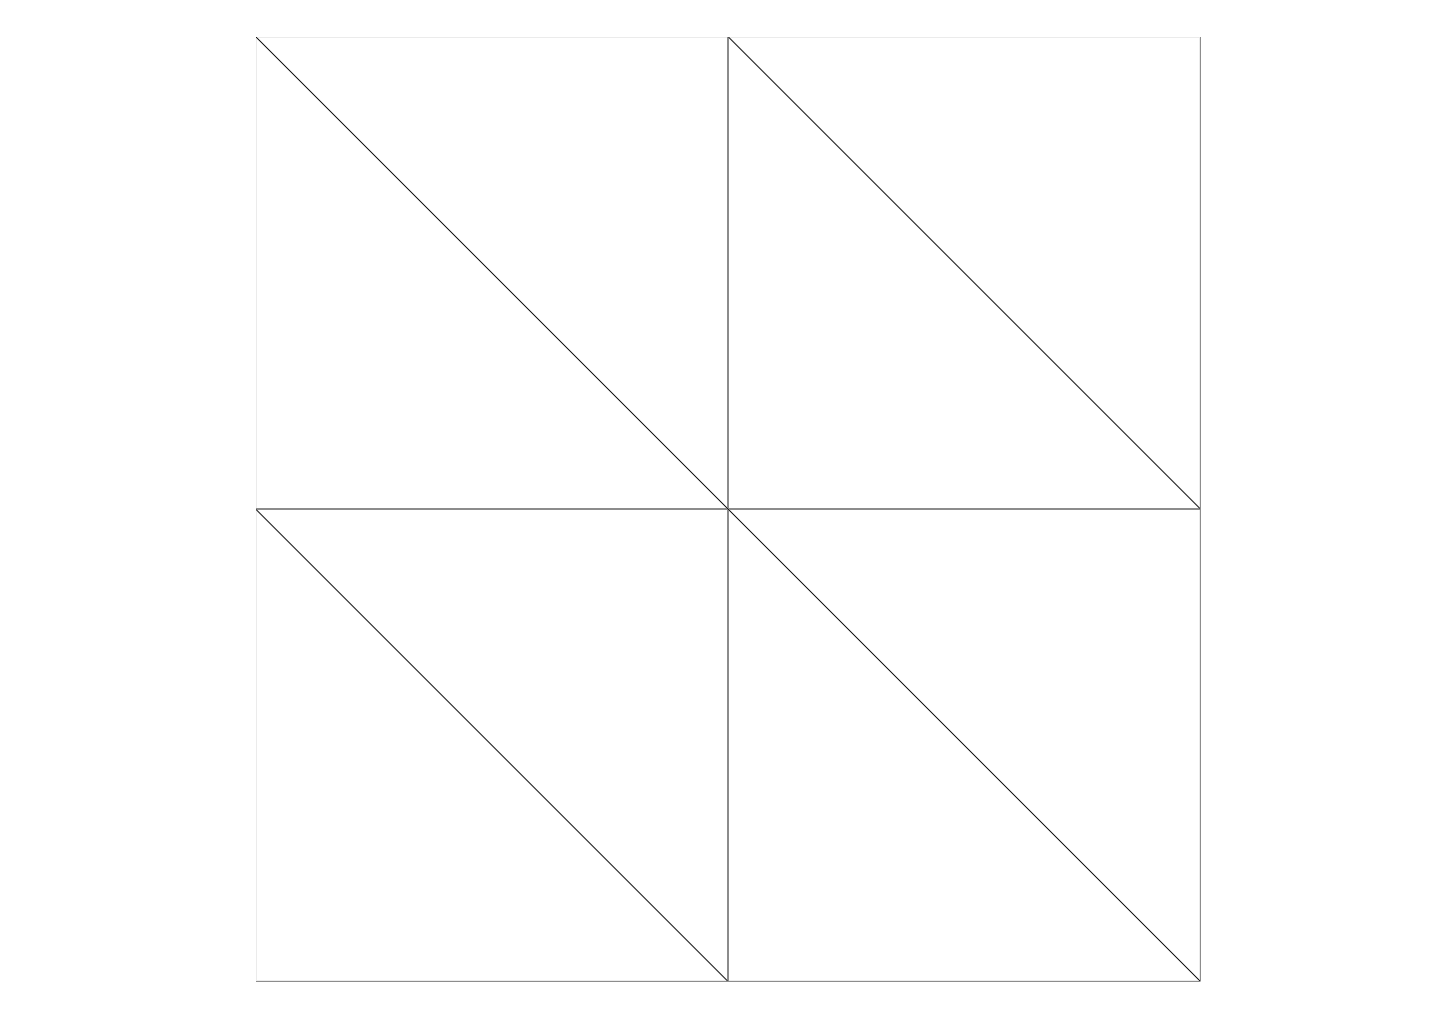
\includegraphics[width=\linewidth]
		{data/synthetic_meshes/square_tesselation_2tri_Dirac_delta_1_v9_f8_wireframe.png}
		\caption{$r=1$, wireframe}\label{fig:sq2.a}
	\end{subfigure}
	\begin{subfigure}[b]{0.32\linewidth}
		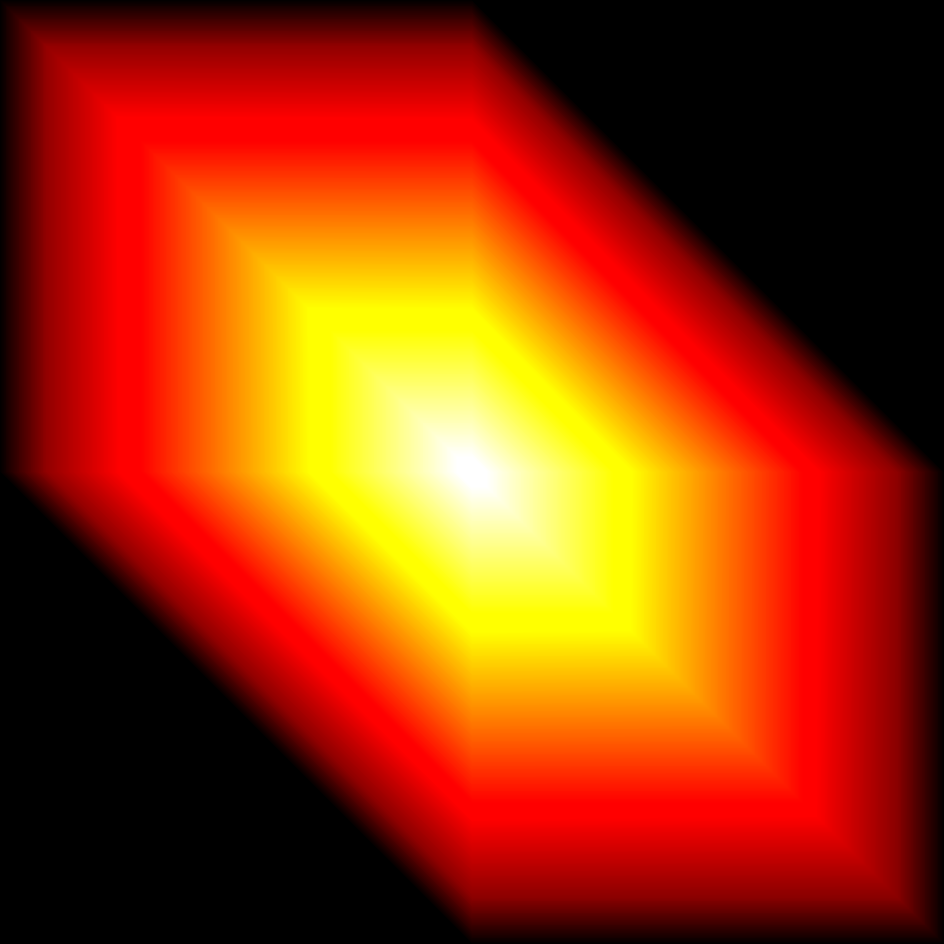
\includegraphics[width=\linewidth]
		{data/synthetic_meshes/square_tesselation_2tri_Dirac_delta_1_v9_f8_funcvals_0iter_crop.png}
		\caption{$r=1$, $c=0$}\label{fig:sq2.b}
	\end{subfigure}
	\begin{subfigure}[b]{0.32\linewidth}
		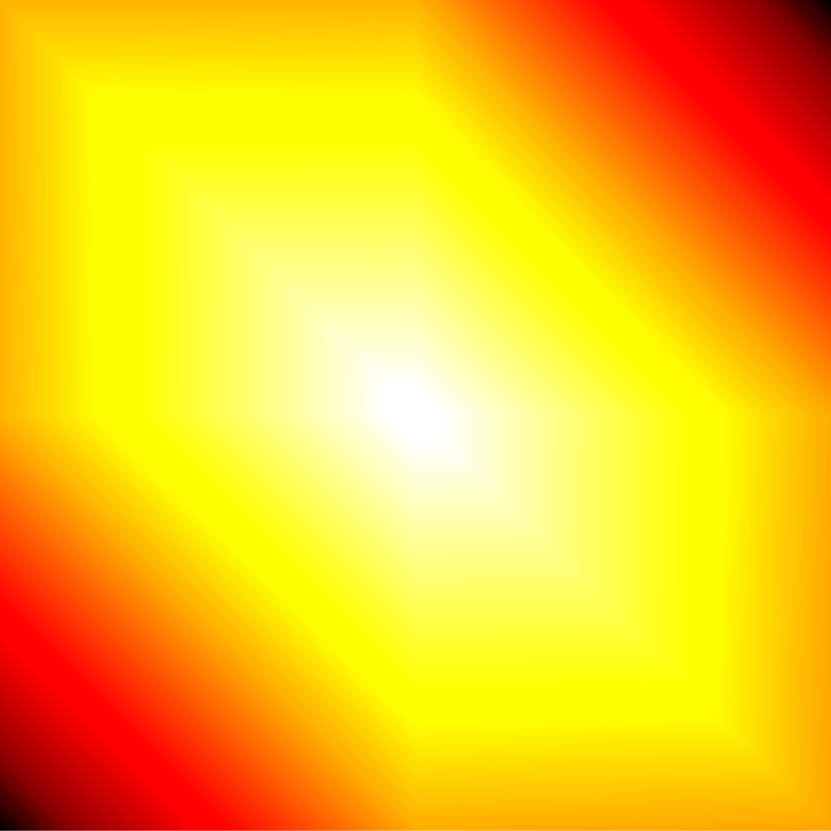
\includegraphics[width=\linewidth]
		{data/synthetic_meshes/square_tesselation_2tri_Dirac_delta_1_v9_f8_funcvals_1iter_crop.png}
		\caption{$r=1$, $c=1$}\label{fig:sq2.c}
	\end{subfigure}

	\bigskip
	\begin{subfigure}[b]{0.32\linewidth}
		
\includegraphics[width=\linewidth]
		{data/synthetic_meshes/square_tesselation_2tri_Dirac_delta_10_v441_f800_wireframe.png}
		\caption{$r=10$, wireframe}\label{fig:sq2.d}
	\end{subfigure}
	\begin{subfigure}[b]{0.32\linewidth}
		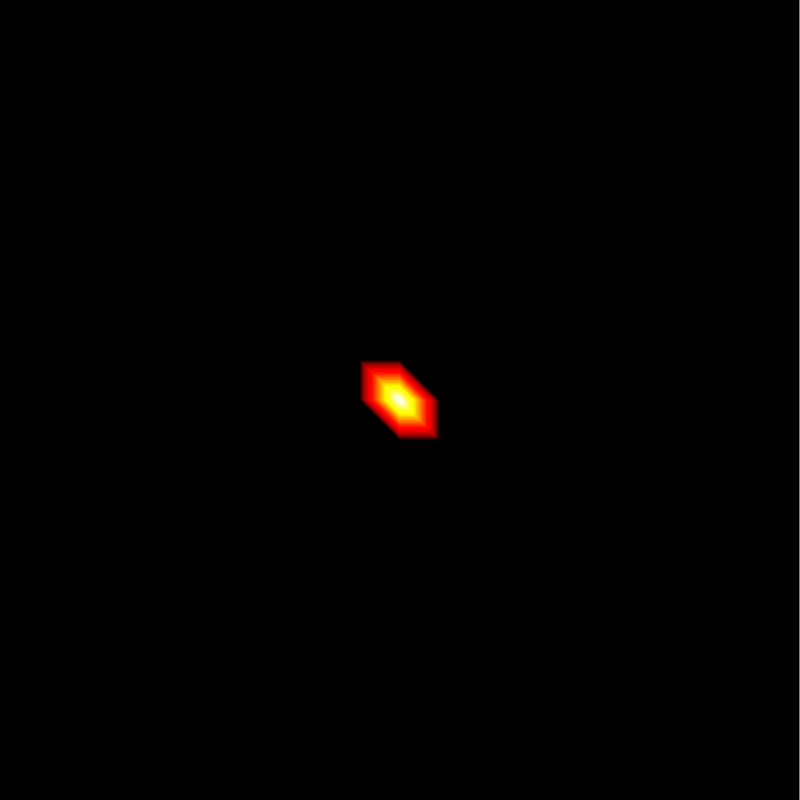
\includegraphics[width=\linewidth]
		{data/synthetic_meshes/square_tesselation_2tri_Dirac_delta_10_v441_f800_funcvals_0iter.png}
		\caption{$r=10$, $c=0$}\label{fig:sq2.e}
	\end{subfigure}
	\begin{subfigure}[b]{0.32\linewidth}
		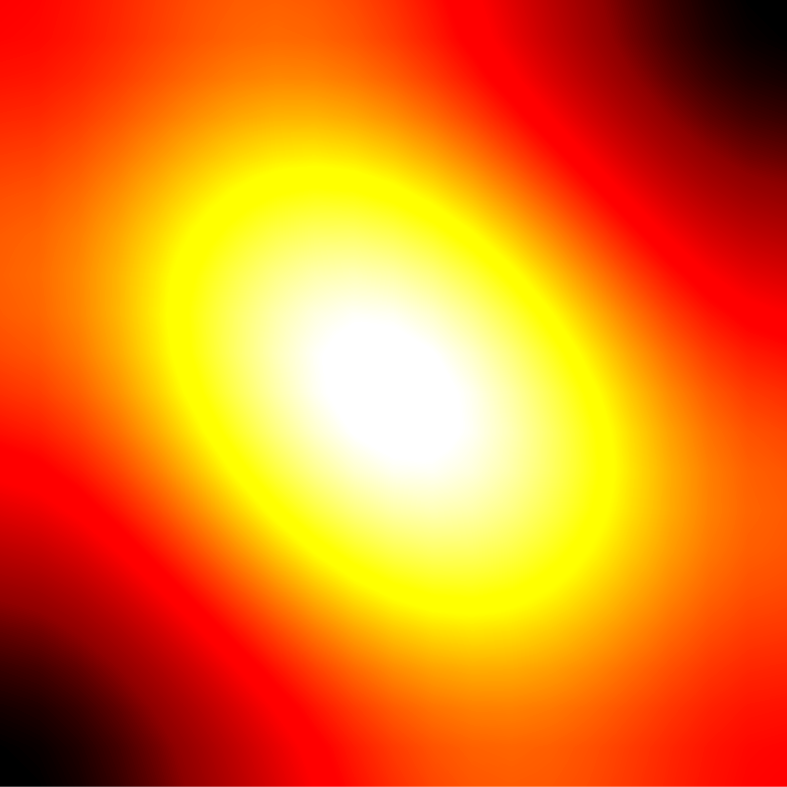
\includegraphics[width=\linewidth]
		{data/synthetic_meshes/square_tesselation_2tri_Dirac_delta_10_v441_f800_funcvals_100iter.png}
		\caption{$r=10$, $c=100$}\label{fig:sq2.f}
	\end{subfigure}
	\caption[Six views, comparing two differently sized of bisected square tessellations]{Comparison of two differently sized bisected square tessellations, generated with parameters $r$ set to 1 and 10: (a) $r=1$ in wireframe (b) $r=1$ colored by function value before convolving the filter (c) $r=1$ colored by function value after convolving the filter once (d) $r=10$ in wireframe (e) $r=10$ colored by function value before convoving the filter (f) $r=10$ colored by function value after convolving the filter 100 times.}
	\label{fig:sq2}
\end{figure}


%
%
%
%
\pagebreak
\subsection{Quadrisected Square Tessellations}
The synthetic mesh generator for quadirsected square tessellations generates meshes characterized by rings of squares around a center point, with the every corner made adjacent to the center point, quadrisecting each square into four equally sized isosceles, right triangles.

The smallest, non-trivial mesh, generated with the parameter $r$ equal to one, is composed of four squares around the center point, represented in total by only thirteen points and sixteen faces, however those numbers grow quickly with increasing parameter size $r$, according to the two equations
\begin{align}
	|\bP| &= 8r^2 + 4r + 1 \\
	|\bT| &= 16r^2
	\label{eq:sq4PointAndFaceCounts}
\end{align}

Figure~\ref{fig:sq2} shows a comparison of two differently sized quadrisected square tessellations, generated with parameters $r$ set to 1 and 10, each in wireframe, shown in (a) and (d), then colored by function value before convolving the filter, shown in (b) and (e), as well as after convolving the filter, once for $r$=1 in (c), and 100 times for $r$=10 in (f). Notice the circular shape of the filter response in part (f).
\todoStyle{sq4 wireframes are not dark enough}

%\begin{figure}[ht]
	\begin{subfigure}[b]{0.32\linewidth}
		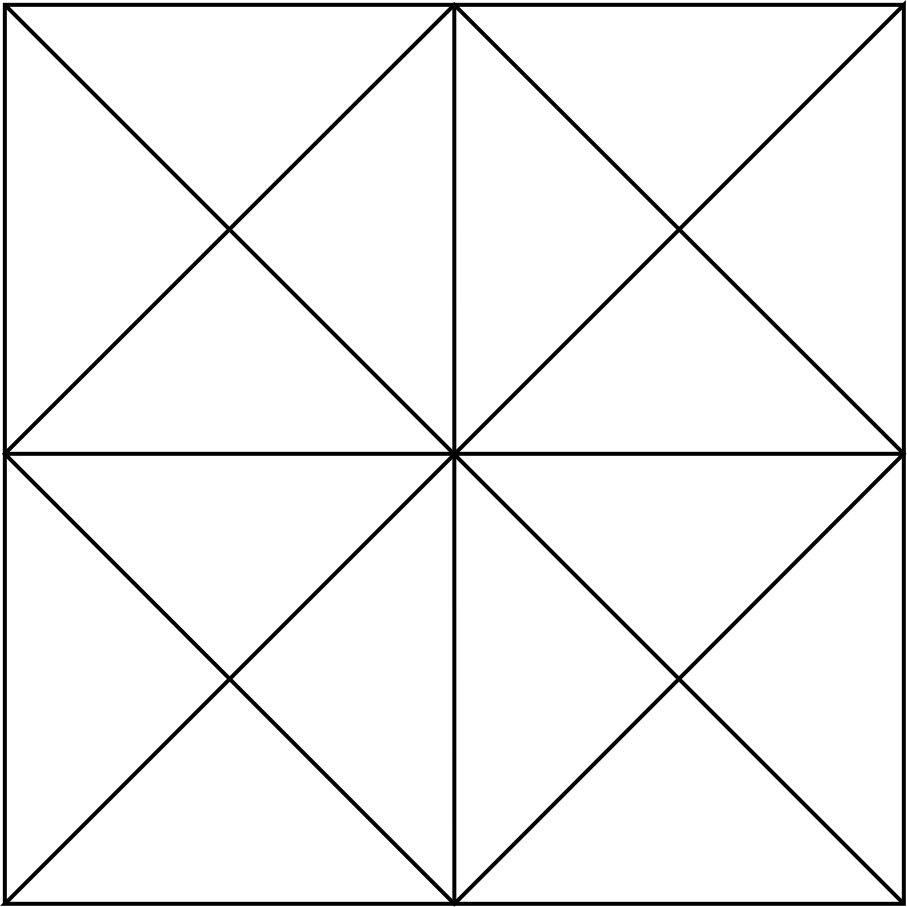
\includegraphics[width=\linewidth]
		{data/synthetic_meshes/square_tesselation_4tri_Dirac_delta_1_v13_f16_wireframe.png}
		\caption{$r=1$, wireframe}\label{fig:sq2.a}
	\end{subfigure}
	\begin{subfigure}[b]{0.32\linewidth}
		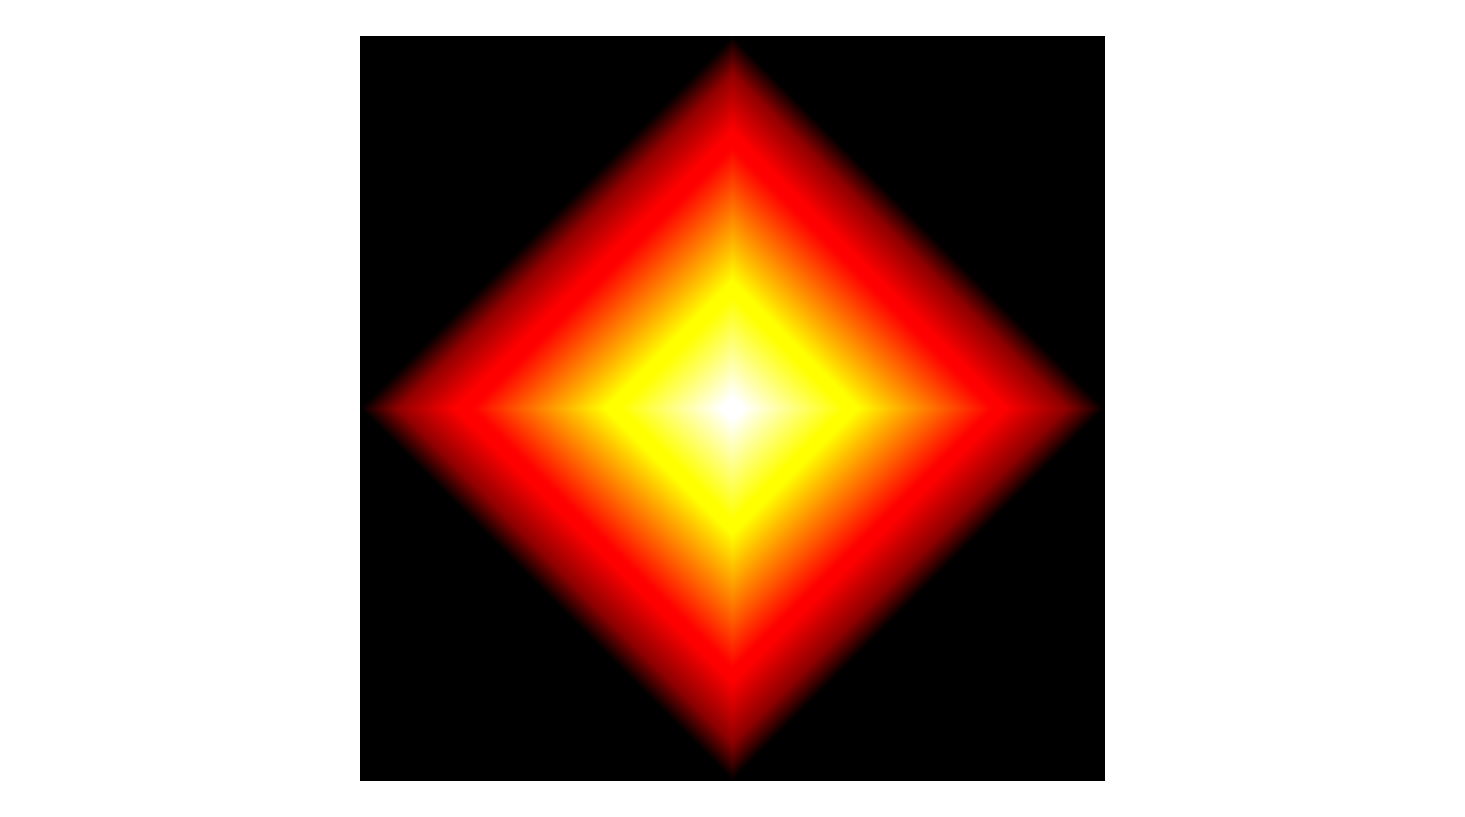
\includegraphics[width=\linewidth]
		{data/synthetic_meshes/square_tesselation_4tri_Dirac_delta_1_v13_f16_funcvals_0iter.png}
		\caption{$r=1$, $c=0$}\label{fig:sq2.b}
	\end{subfigure}
	\begin{subfigure}[b]{0.32\linewidth}
		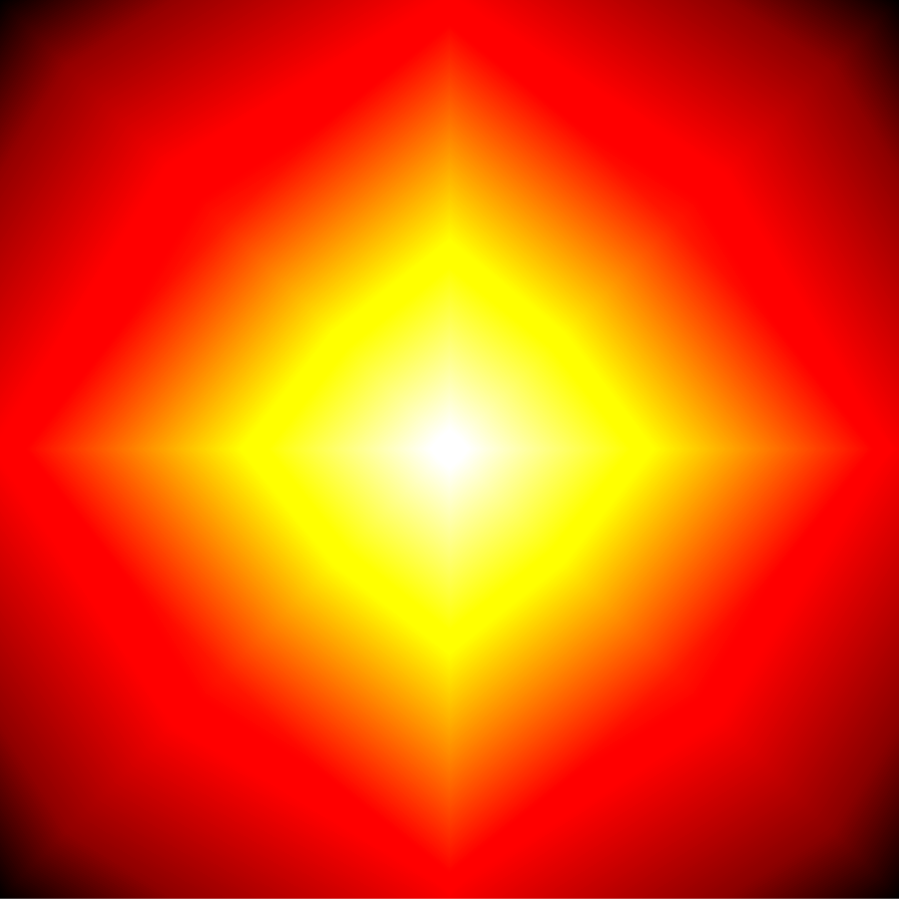
\includegraphics[width=\linewidth]
		{data/synthetic_meshes/square_tesselation_4tri_Dirac_delta_1_v13_f16_funcvals_1iter.png}
		\caption{$r=1$, $c=1$}\label{fig:sq2.c}
	\end{subfigure}

	\bigskip
	\begin{subfigure}[b]{0.32\linewidth}
		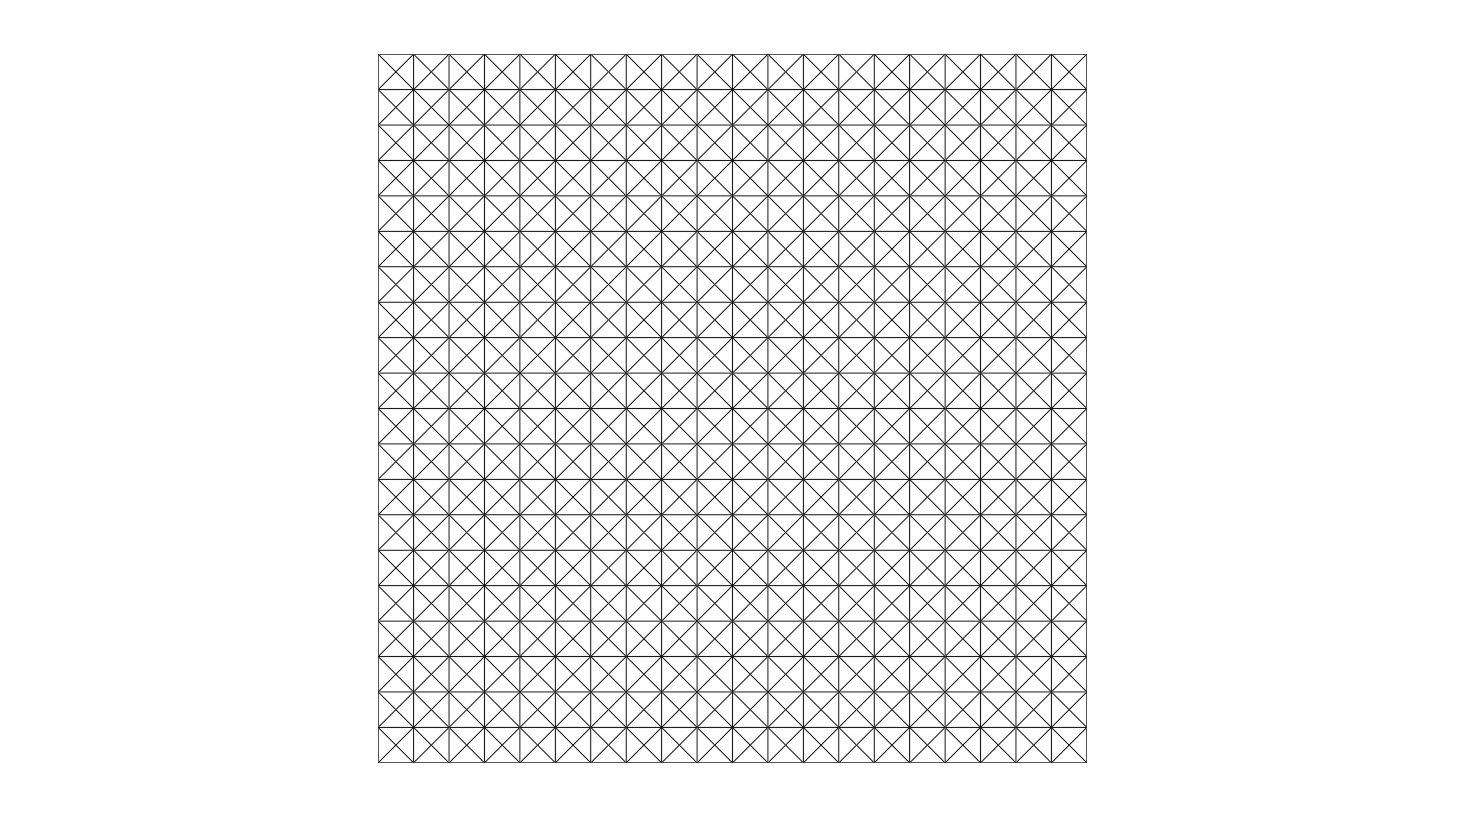
\includegraphics[width=\linewidth]
		{data/synthetic_meshes/square_tesselation_4tri_Dirac_delta_10_v841_f1600_wireframe.png}
		\caption{$r=10$, wireframe}\label{fig:sq2.d}
	\end{subfigure}
	\begin{subfigure}[b]{0.32\linewidth}
		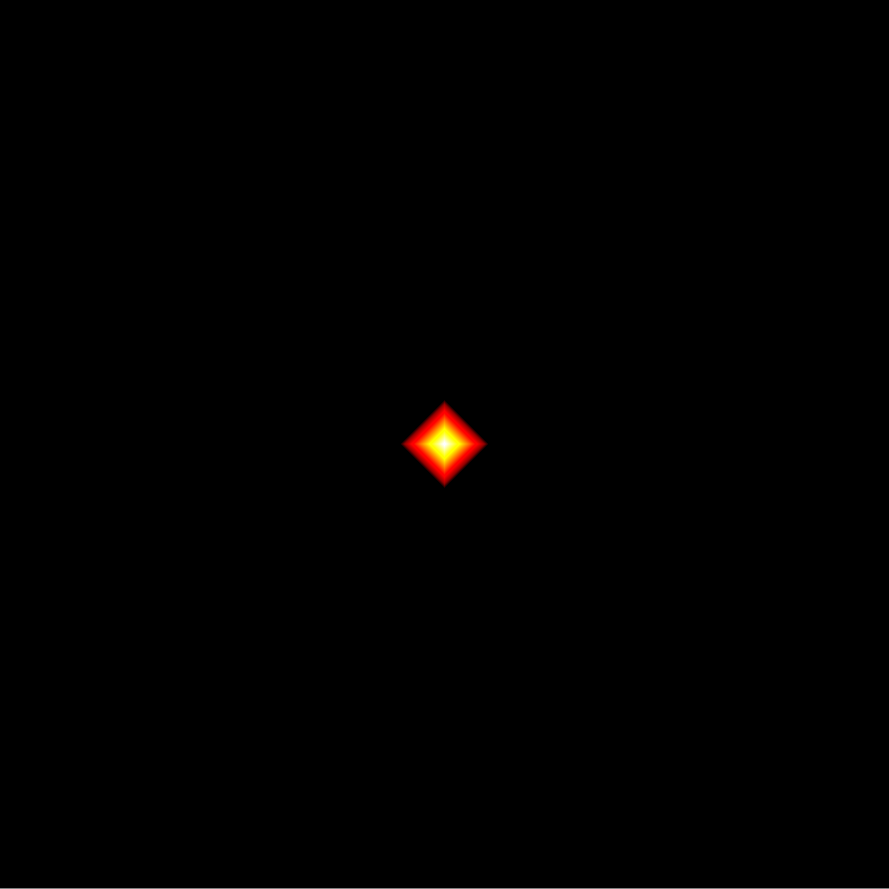
\includegraphics[width=\linewidth]
		{data/synthetic_meshes/square_tesselation_4tri_Dirac_delta_10_v841_f1600_funcvals_0iter.png}
		\caption{$r=10$, $c=0$}\label{fig:sq2.e}
	\end{subfigure}
	\begin{subfigure}[b]{0.32\linewidth}
		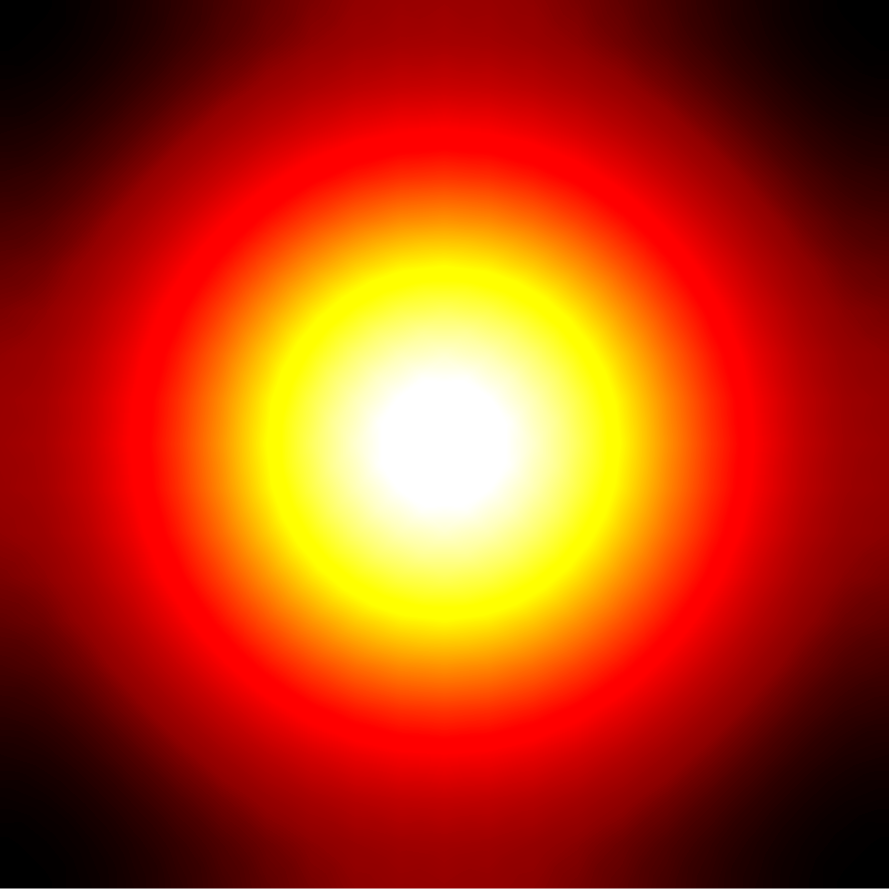
\includegraphics[width=\linewidth]
		{data/synthetic_meshes/square_tesselation_4tri_Dirac_delta_10_v841_f1600_funcvals_100iter.png}
		\caption{$r=10$, $c=100$}\label{fig:sq2.f}
	\end{subfigure}
	\caption[Six views, comparing two differently sized of quadirsected square tessellations]{Comparison of two differently sized quadirsected square tessellations, generated with parameters $r$ set to 1 and 10: (a) $r=1$ in wireframe (b) $r=1$ colored by function value before convolving the filter (c) $r=1$ colored by function value after convolving the filter once (d) $r=10$ in wireframe (e) $r=10$ colored by function value before convoving the filter \newline(f) $r=10$ colored by function value after convolving the filter 100 times.}
	\label{fig:sq2}
\end{figure}


%
%
%
%
\pagebreak
\subsection{Hexagonal Tesselation}
The synthetic mesh generator for hexagonal tessellations generates meshes characterized by hexagons around one central hexagon, with each corner of the hexagons made adjacent to its own center point, creating six equilateral triangles per hexagon, and ensuring that every edge lengths in the mesh is of equal size.

The smallest, non-trivial mesh, generated with the parameter $r$ equal to zero, is composed of one hexagon around the center point, represented in total by only seven points and six faces, however those numbers grow quickly with increasing parameter size $r$, according to the two equations
\begin{align}
	|\bP| &= 3r^2 + 3r + 7 +\sum_{i=1}^r{6(2i + 1)}\\
	|\bT| &= 18r^2 + 18r + 6
	\label{eq:hexPointAndFaceCounts}
\end{align}

Figure~\ref{fig:sq2} shows a comparison of two differently sized hexagonal tessellations, generated with parameters $r$ set to 1 and 10, each in wireframe, shown in (a) and (d), then colored by function value before convolving the filter, shown in (b) and (e), as well as after convolving the filter, once for $r=1$ in (c), and 200 times for $r=10$ in (f).
\todoStyle{b c e and f need to correct for dpi}
%\begin{figure}[ht]
	\begin{subfigure}[b]{0.32\linewidth}
		
\includegraphics[width=\linewidth]
		{data/synthetic_meshes/hexagonal_tessellation_Dirac_delta_1_v31_f42_wireframe.png}
		\caption{$r=1$, wireframe}\label{fig:hex.a}
	\end{subfigure}
	\begin{subfigure}[b]{0.32\linewidth}
		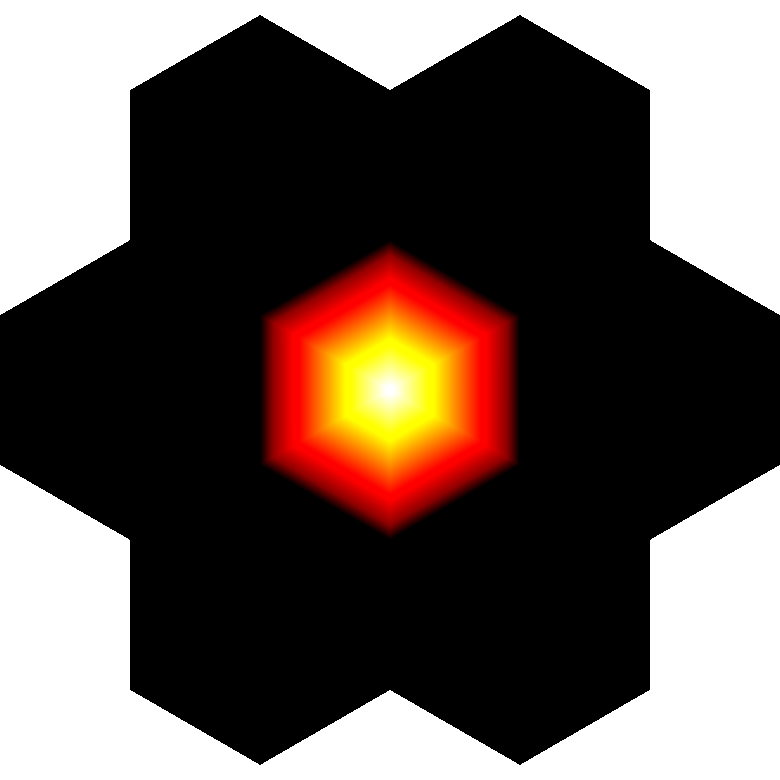
\includegraphics[width=\linewidth]
		{data/synthetic_meshes/hexagonal_tessellation_Dirac_delta_1_v31_f42_funcvals_0iter_crop.png}
		\caption{$r=1$, $c=0$}\label{fig:hex.b}
	\end{subfigure}
	\begin{subfigure}[b]{0.32\linewidth}
		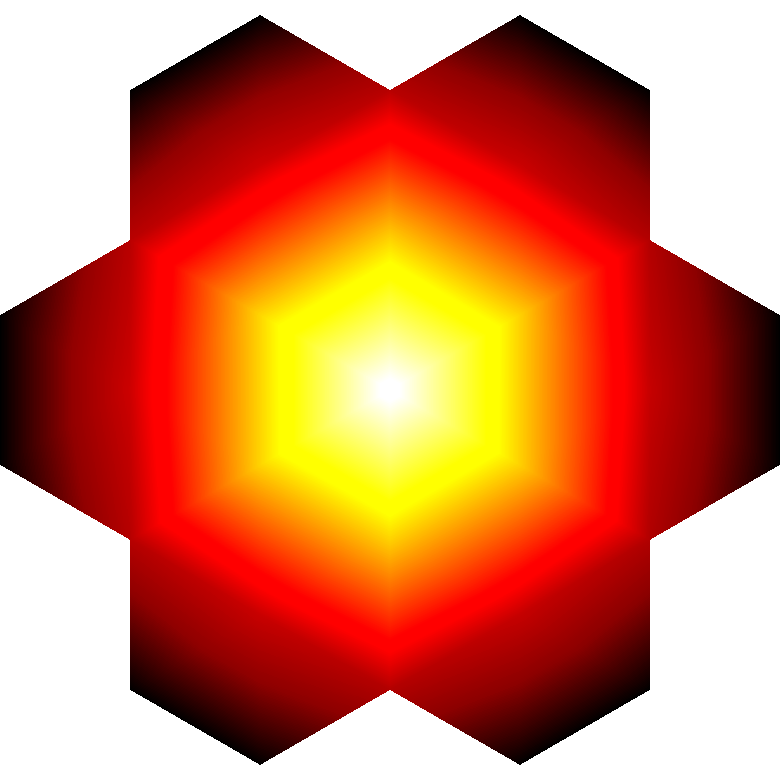
\includegraphics[width=\linewidth]
		{data/synthetic_meshes/hexagonal_tessellation_Dirac_delta_1_v31_f42_funcvals_2iter_crop.png}
		\caption{$r=1$, $c=2$}\label{fig:hex.c}
	\end{subfigure}

	\begin{subfigure}[b]{0.32\linewidth}
		
\includegraphics[width=\linewidth]
		{data/synthetic_meshes/hexagonal_tessellation_Dirac_delta_10_v1057_f1986_wireframe.png}
		\caption{$r=10$, wireframe}\label{fig:hex.d}
	\end{subfigure}
	\begin{subfigure}[b]{0.32\linewidth}
		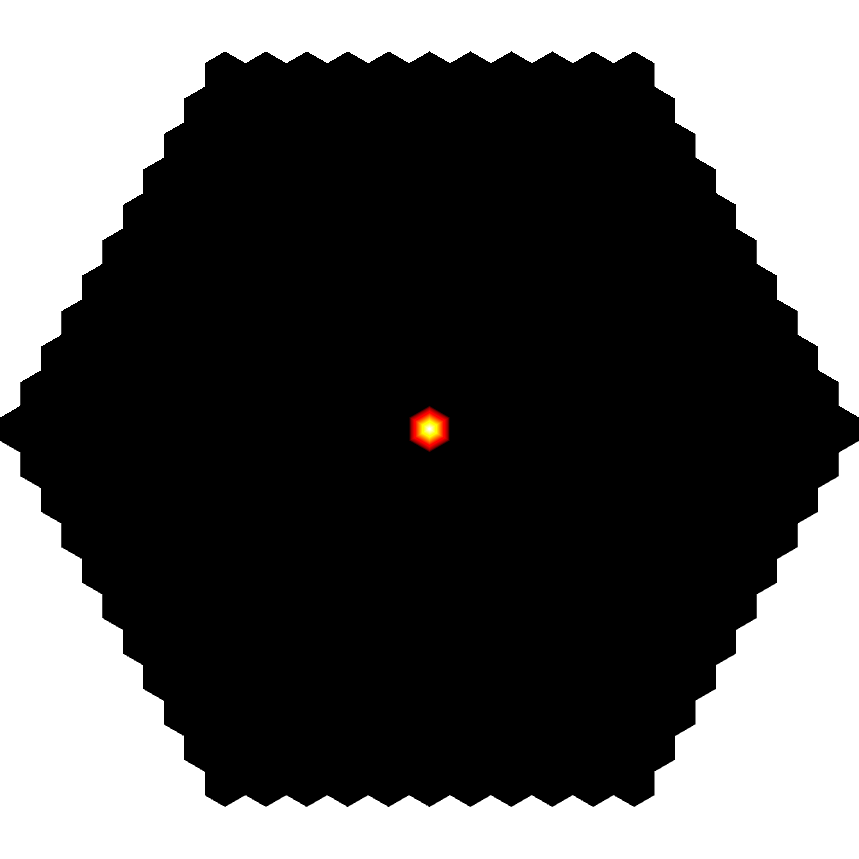
\includegraphics[width=\linewidth]
		{data/synthetic_meshes/hexagonal_tessellation_Dirac_delta_10_v1057_f1986_funcvals_0iter_crop.png}
		\caption{$r=10$, $c=0$}\label{fig:hex.e}
	\end{subfigure}
	\begin{subfigure}[b]{0.32\linewidth}
		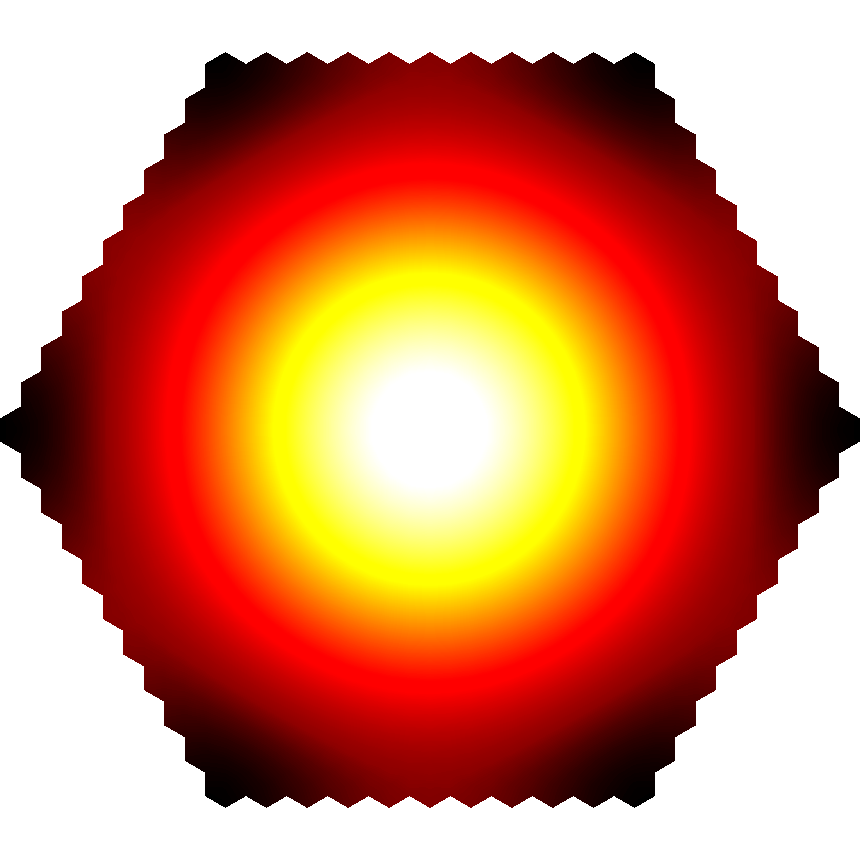
\includegraphics[width=\linewidth]
		{data/synthetic_meshes/hexagonal_tessellation_Dirac_delta_10_v1057_f1986_funcvals_200iter_crop.png}
		\caption{$r=10$, $c=200$}\label{fig:hex.f}
	\end{subfigure}
	\caption[Six Views Comparing Hexagonal Tessellations]{Comparison of two differently-sized, hexagonal tessellations, generated with parameters $r$ set to 1 and 10. (a) $r=1$ in wireframe, (b) $r=1$ colored by function value before convolving the filter, (c) $r=1$ colored by function value after convolving the filter once, (d) $r=10$ in wireframe, (e) $r=10$ colored by function value before convoving the filter, and (f) $r=10$ colored by function value after convolving the filter 200 times.}
	\label{fig:hex}
\end{figure}


%
%
%
%
\pagebreak
\subsection{Random Triangulated Discs}
The synthetic mesh generator for random triangulated discs generates meshes characterized by radially bounded, uniformly distributed, random meshes; including one point located at the origin. Furthermore, the points are then triangulated following the well-studied method originally presented by of Delaunay~\cite{Delaunay34}.
\todoResearch{how are the points uniformly distributed?}

Unlike the other generators, random triangulated discs requires two parameters, the radius of the disc $r$, and the explicit number of points $p$. For our experiments, the parameters were chosen to ensure parity with the sizes and point density of the other synthetic meshes.
%, the following table of parameters where used.
%\begin{table}[ht]
%\begin{tabular}{rrr}
%\textbf{R} & \textbf{Points} & \textbf{Faces} \\
%\hline
%1	11
%3	67
%10	641
%30	5521
%100	60401
%300	541201
%1000	6004001
%3000	54012001

%   0 &          7 &           6\\
%    1 &         31 &          42\\
%    3 &        133 &         222\\
%   10 &      1,057 &       1,986\\
%   30 &      8,557 &      16,746\\
%  100 &     91,507 &     181,806\\
%  300 &    814,507 &   1,625,406\\
%1,000 &  9,015,007 &  18,018,006\\
%3,000 & 81,045,007 & 162,054,006%
%\caption{Summary of the Counts of Points and Faces for Increasing Parameters of the Hexagonal Tesselation Synthetic Mesh Generator\label{tbl:hex}}
%\end{tabular}
%\end{table}

%The smallest, non-trivial mesh, generated with the parameter $r$ equal to one, is composed of one hexagon around the center point, represented in total by only seven points and 6 faces, however those numbers grow quickly with increasing parameter size $r$, according to the two equations
%\begin{align}
%	|\bP| &= 3r^2 + 3r + 7 +\sum_{r=1}^r{6(2r + 1)}\\
%	|\bT| &= 18r^2 + 18r + 6
%	\label{eq:hexPointAndFaceCounts}
%\end{align}

Figure~\ref{fig:sq2} shows a comparison of two differently sized, random triangulated discs, generated with parameters $r$ set to 1 and 10, and parameters $p$ set to 11 and 641, each in wireframe, shown in (a) and (d), then colored by function value before convolving the filter, shown in (b) and (e), as well as after convolving the filter, twice for $r=1$ in (c), and 10,000 times for $r=10$ in (f). Notice in (f), the relatively high number of iterations required required to achieve the shown filter response.

%\begin{figure}[ht]
	\begin{subfigure}[b]{0.32\linewidth}
		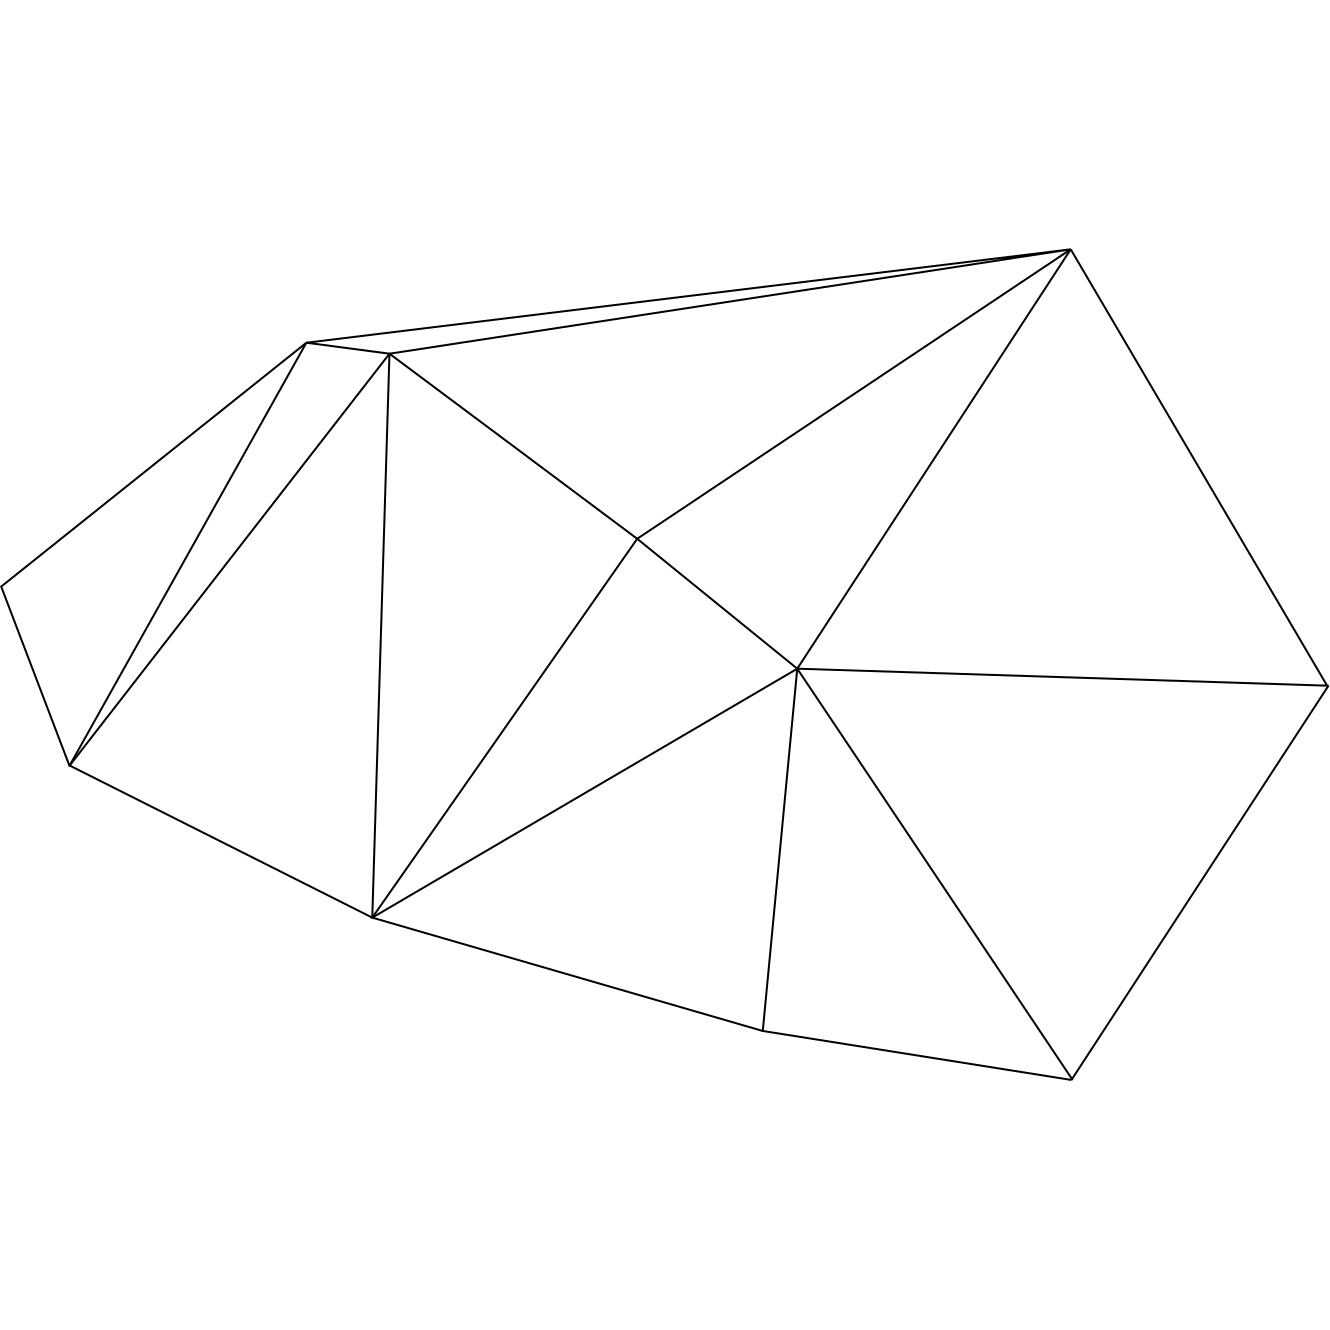
\includegraphics[width=\linewidth]
		{data/synthetic_meshes/random_circle_tessellation_Dirac_delta_1_v11_f12_wireframe.png}
		\caption{$r=1$, $p=11$, wireframe}\label{fig:rcirc.a}
	\end{subfigure}
	\begin{subfigure}[b]{0.32\linewidth}
		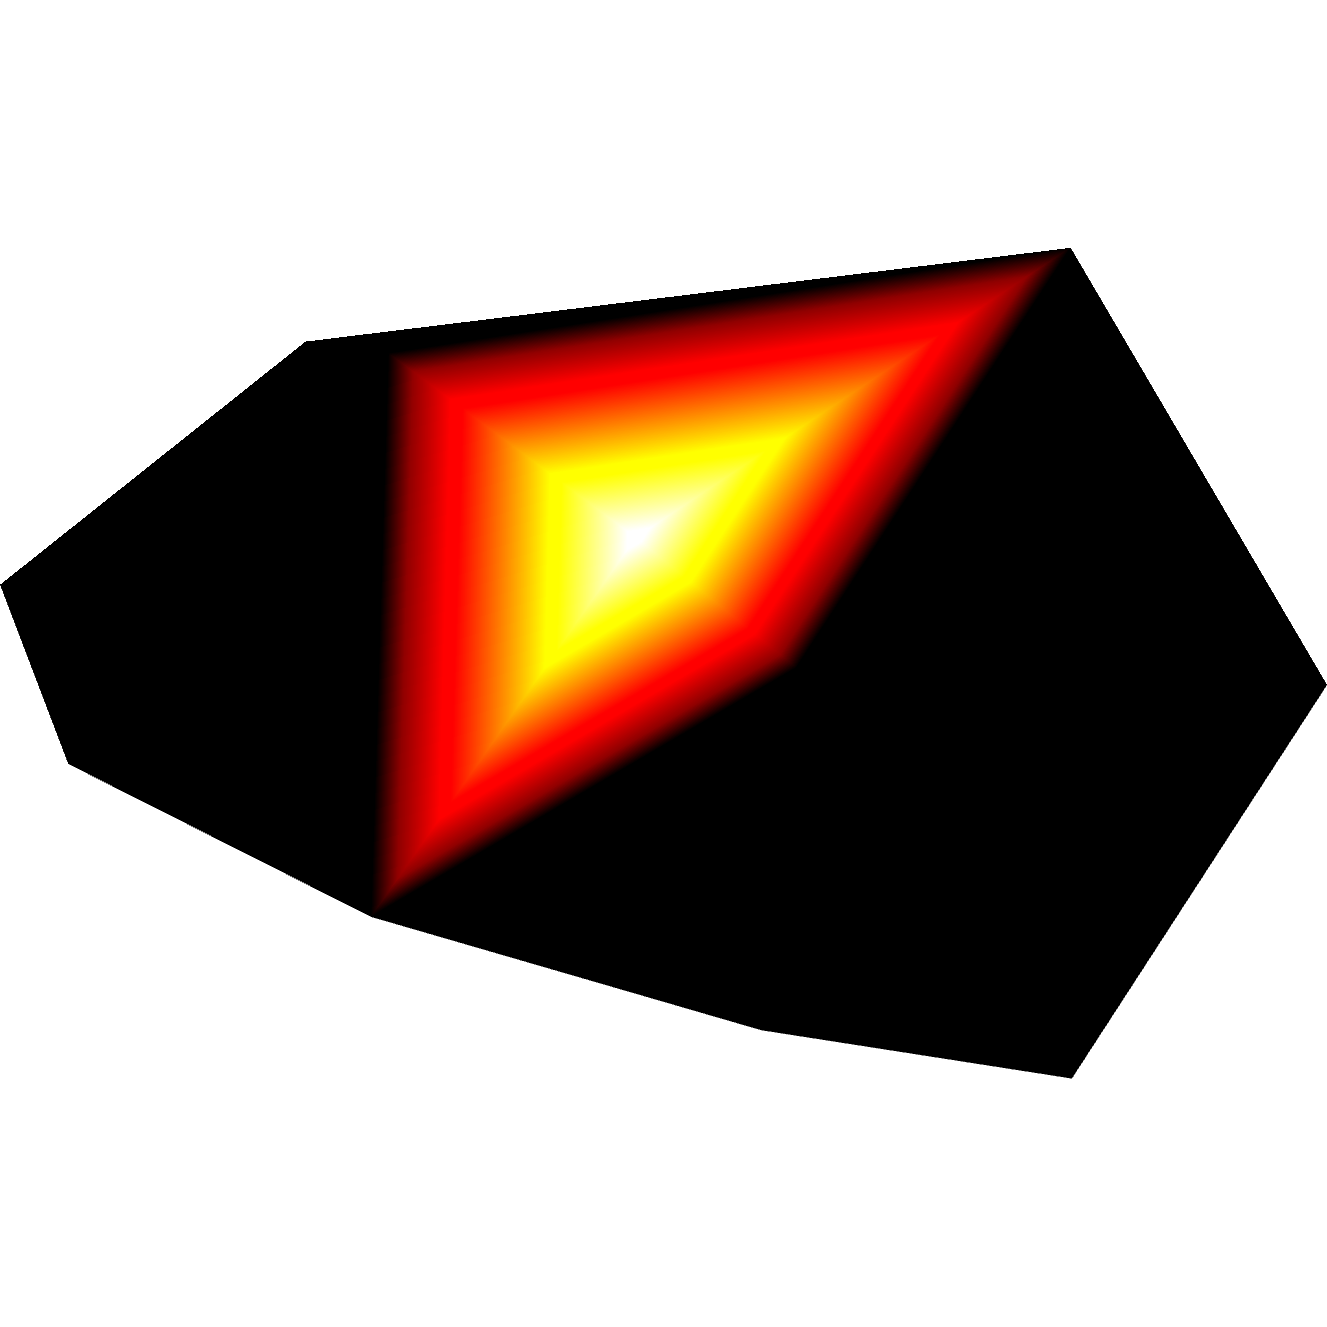
\includegraphics[width=\linewidth]
		{data/synthetic_meshes/random_circle_tessellation_Dirac_delta_1_v11_f12_funcvals_0iter.png}
		\caption{$r=1$, $p=11$, $c=0$}\label{fig:rcirc.c}
	\end{subfigure}
	\begin{subfigure}[b]{0.32\linewidth}
		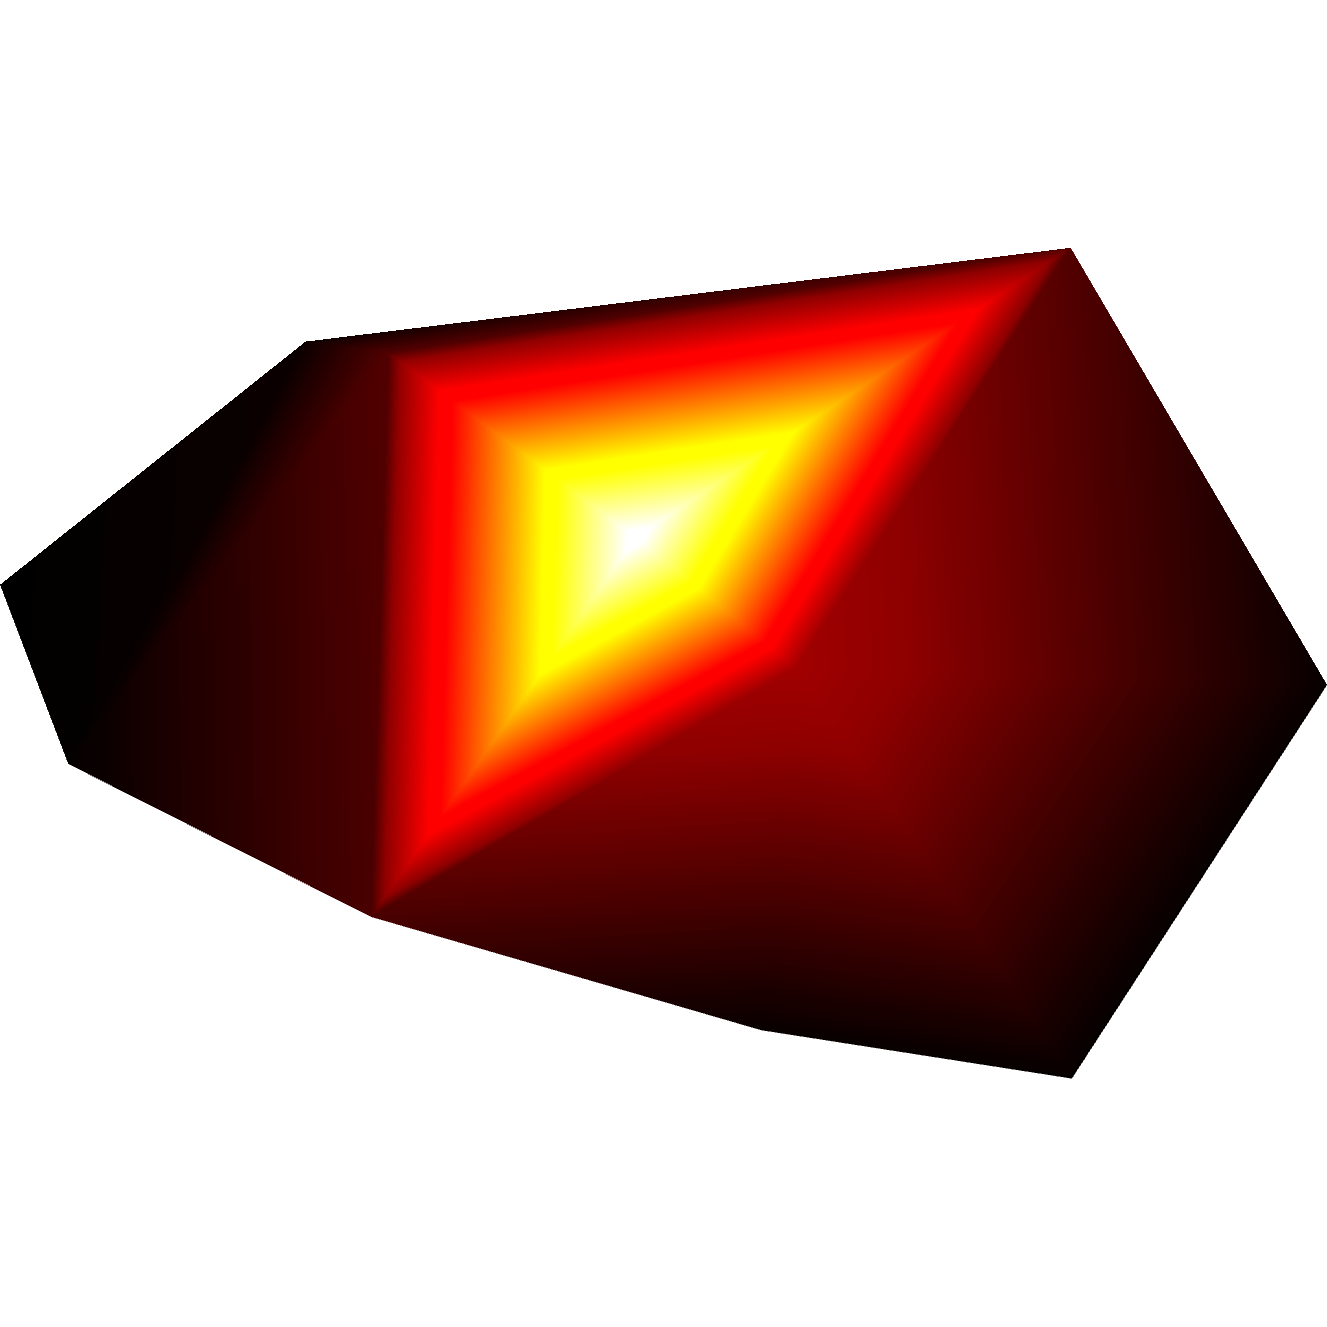
\includegraphics[width=\linewidth,]
		{data/synthetic_meshes/random_circle_tessellation_Dirac_delta_1_v11_f12_funcvals_2iter.png}
		\caption{$r=1$, $p=11$, $c=2$}\label{fig:rcirc.e}
	\end{subfigure}

	\bigskip
	\begin{subfigure}[b]{0.32\linewidth}
		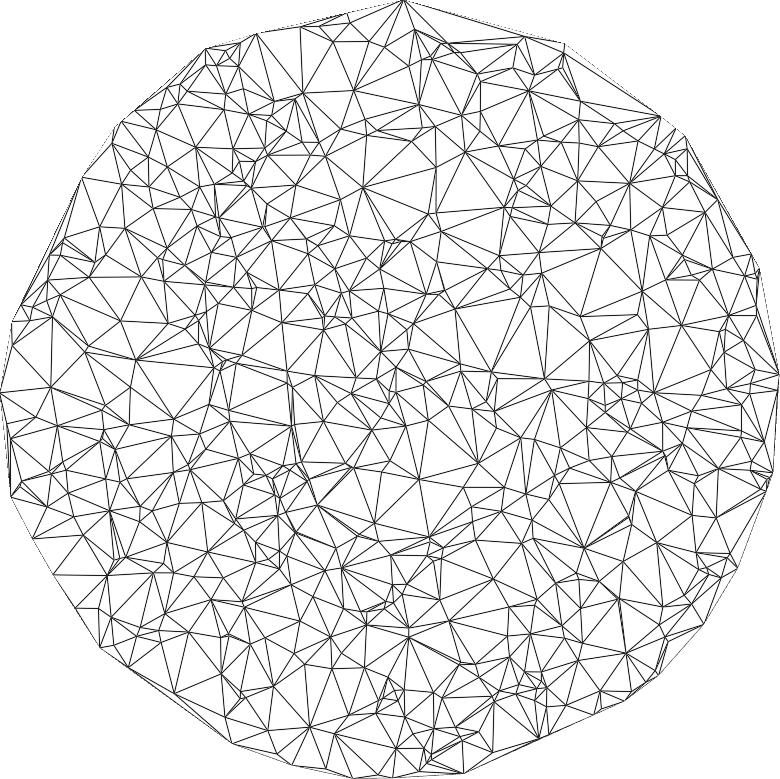
\includegraphics[width=\linewidth]
		{data/synthetic_meshes/random_circle_tessellation_Dirac_delta_10_v641_f1252_wireframe.png}
		\caption{$r=10$, $p=641$, wireframe}\label{fig:rcirc.b}
	\end{subfigure}
	\begin{subfigure}[b]{0.32\linewidth}
		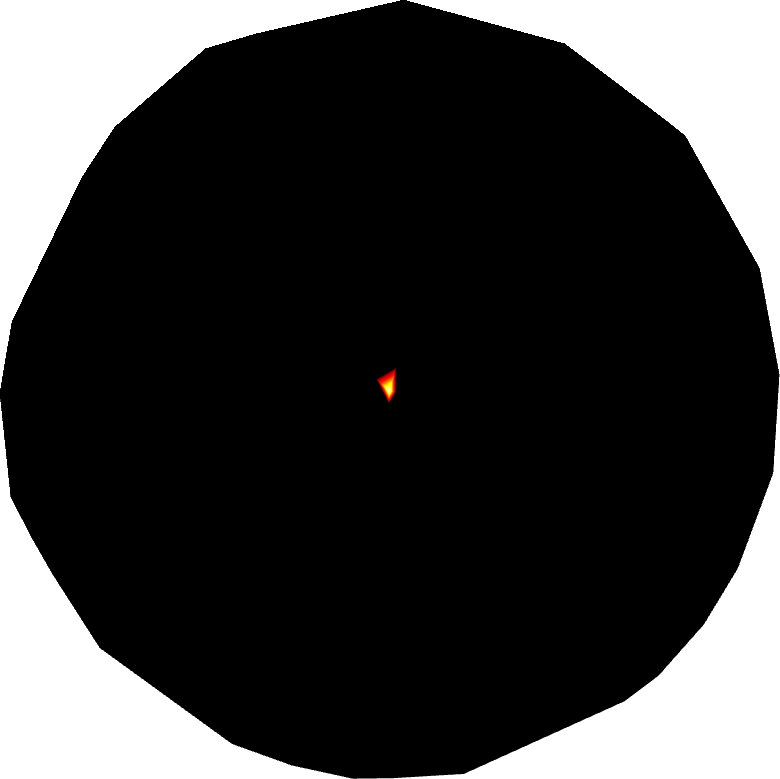
\includegraphics[width=\linewidth]
		{data/synthetic_meshes/random_circle_tessellation_Dirac_delta_10_v641_f1252_funcvals_0iter.png}
		\caption{$r=10$, $p=641$, $c=0$}\label{fig:rcirc.d}
	\end{subfigure}
	\begin{subfigure}[b]{0.32\linewidth}
		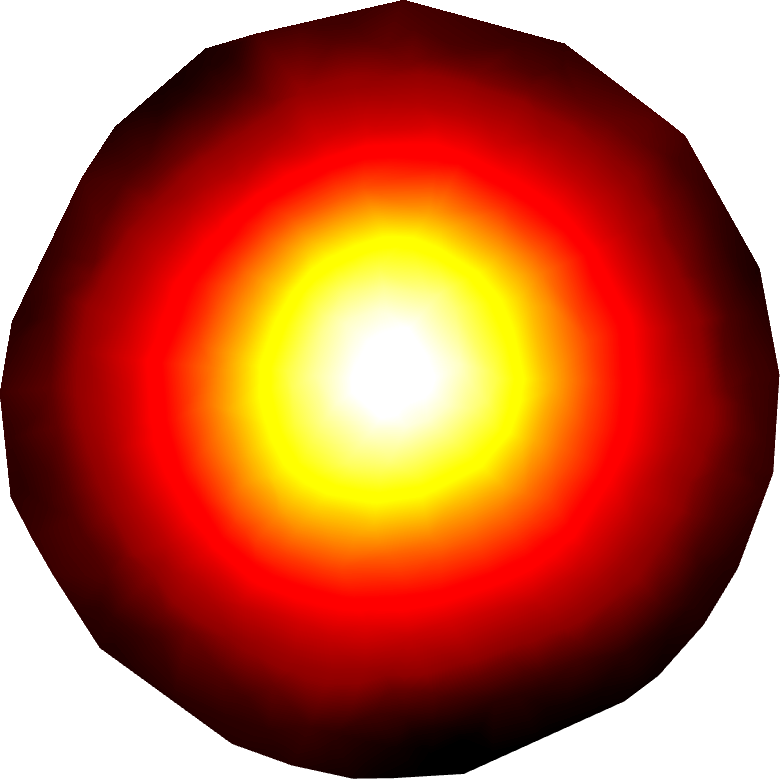
\includegraphics[width=\linewidth]
		{data/synthetic_meshes/random_circle_tessellation_Dirac_delta_10_v641_f1252_funcvals_10000iter.png}
		\caption{$r=10$, $p=641$, $c=10^4$}\label{fig:rcirc.f}
	\end{subfigure}
	\caption[Six views, comparing two differently sized, random triangulated discs]{Comparison of two differently sized, random triangulated discs, generated with parameters $r$ set to 1 and 10, and parameters $p$ set to 11 and 641: (a) $r=1$, $p=11$ in wireframe (b) $r=1$, $p=11$ colored by function value before convolving the filter (c) $r=1$, $p=11$ colored by function value after convolving the filter twice (d) $r=10$, $p=641$ in wireframe (e) $r=10$, $p=641$ colored by function value before convoving the filter (f) $r=10$, $p=641$ colored by function value after convolving the filter 10,000 times.}
	\label{fig:rdisc}
\end{figure}



%
%
%
%
%
%
\pagebreak
\section{Acquired \tdd{}}
\dots
Each acquired mesh was processed using the GigaMesh framework to generate the function values using the MSII, Multi-Scale Integral Invariants filter\todoCitation{}

%
%
%
%
\pagebreak
\subsection{University of Heidelberg Seal}
The seal of the University of Heidelberg, established 1386, as stored by the Univeristy of Heidelberg Archives. Captured with a high resolution 3D-scanner, with the raw scanned data stored in the heiDATA dataverse of the IWR Computer Graphics~\cite{Unisiegel}. This partial model is taken from the center of the original data, and is comprised of 397,210 points and 789,406 faces.

Figure~\ref{fig:unisiegel} shows\dots
\begin{figure}[ht]
	\begin{subfigure}[b]{0.32\linewidth}
		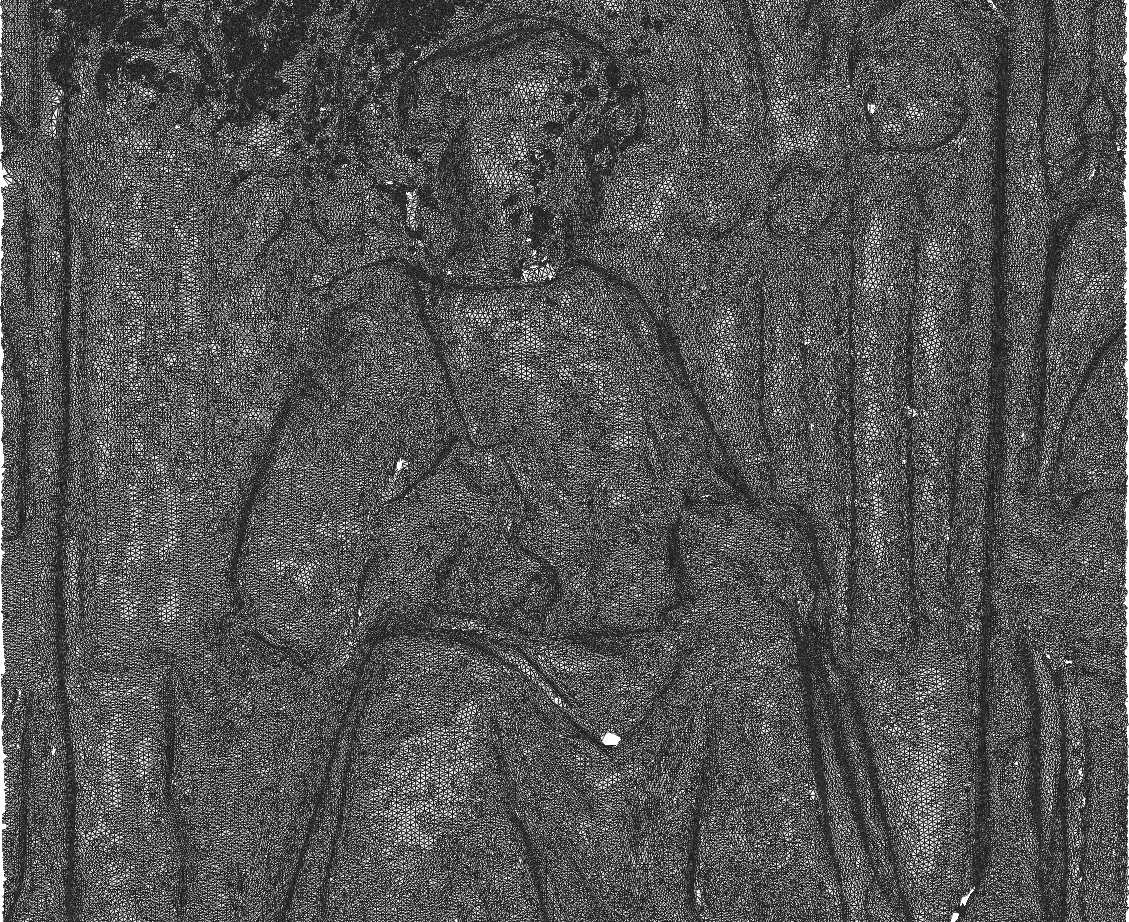
\includegraphics[width=\linewidth]{data/acquired_meshes/unisiegel_wireframe.png}
		\caption{wireframe}\label{fig:unisiegel.a}
	\end{subfigure}
	\begin{subfigure}[b]{0.32\linewidth}
		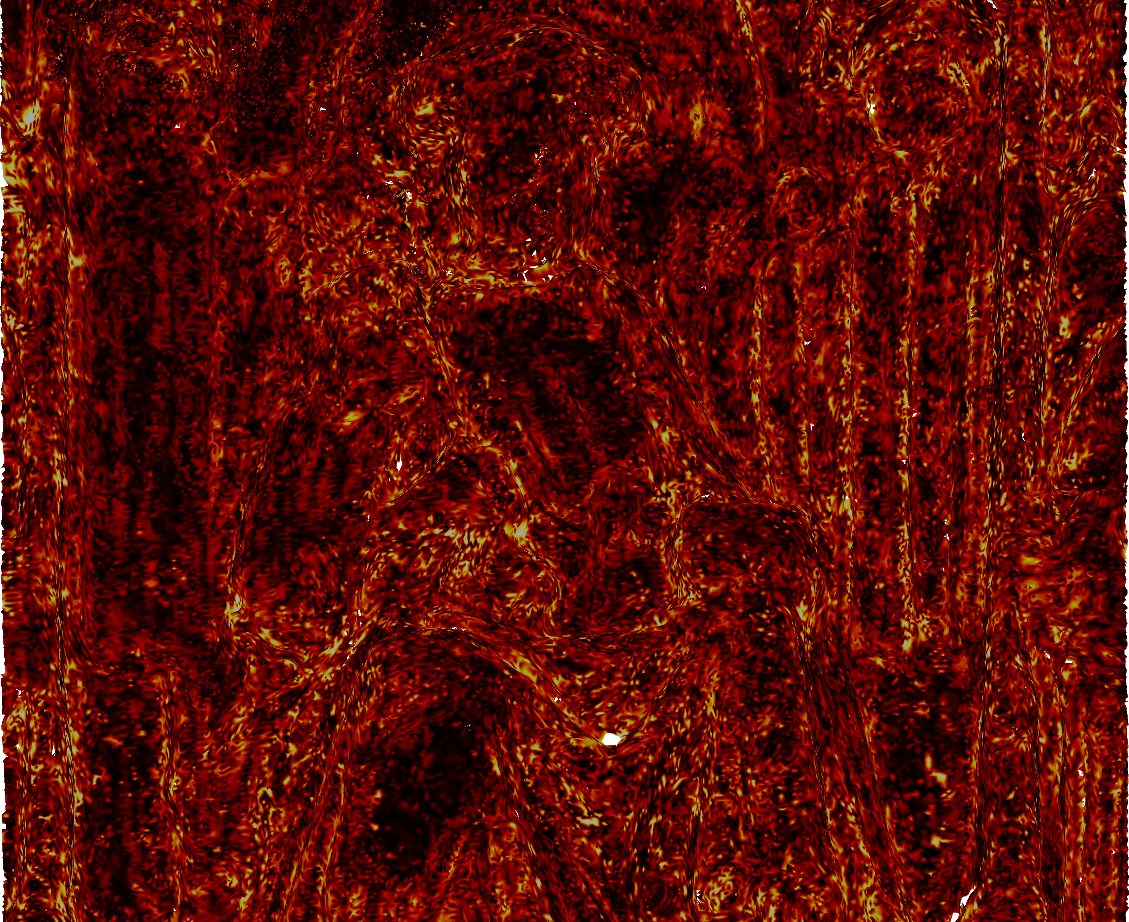
\includegraphics[width=\linewidth]{data/acquired_meshes/unisiegel_0iter.png}
		\caption{$c=0$}\label{fig:unisiegel.b}
	\end{subfigure}
	\begin{subfigure}[b]{0.32\linewidth}
		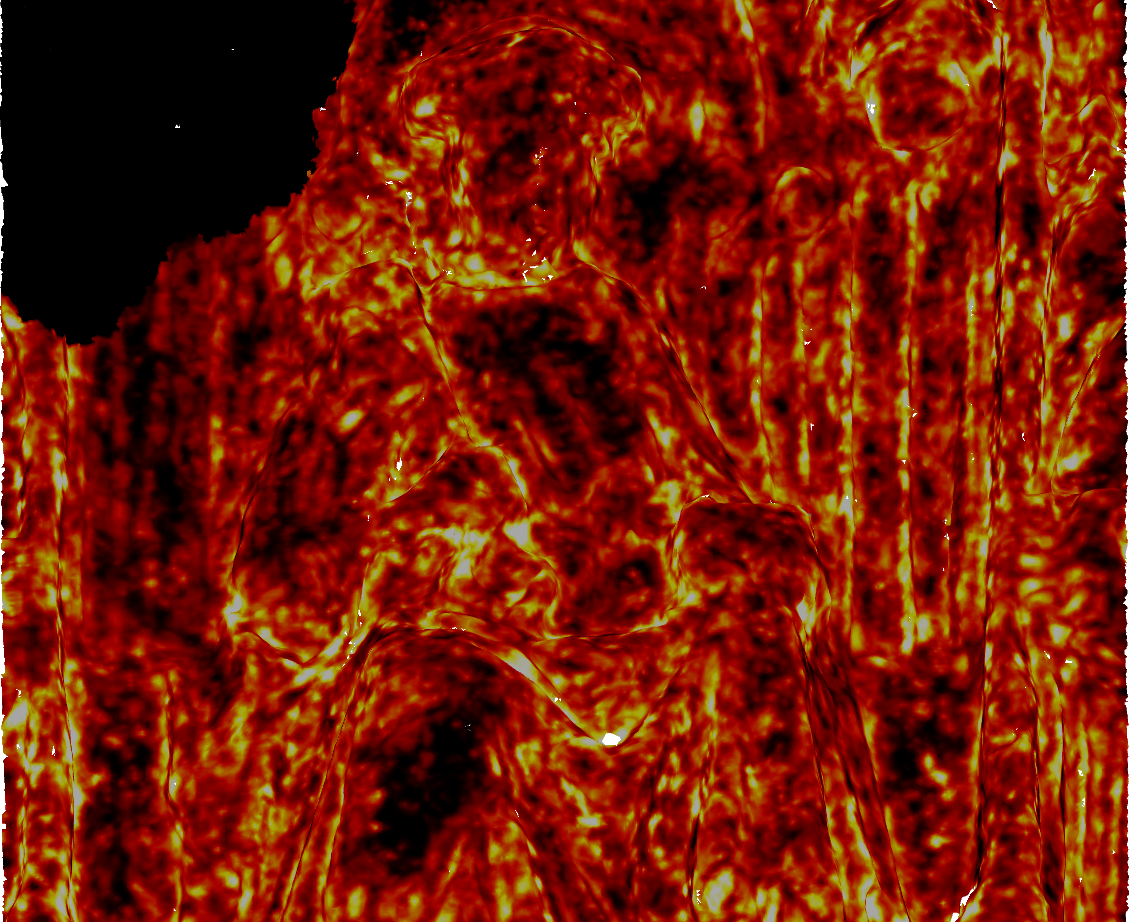
\includegraphics[width=\linewidth]{data/acquired_meshes/unisiegel_100iter.png}
		\caption{$c=100$}\label{fig:unisiegel.c}
	\end{subfigure}
	\caption[Three views of the Univeristy of Heidelberg Seal]{Three views of the Univeristy of Heidelberg seal (a) in wireframe, (b) colored by \gls{tMSIIf} value before convolving the filter, (c) colored by function value after convolving the filter 100 times.}
	\label{fig:unisiegel}
\end{figure}


%
%
%
%
\subsection{A Flat surface}
Flat surfaces have NOISE!
Figure~\ref{fig:ILATO}: ILATO\_1A\_SM2066-HE5-60\_070214\_merged\_GMO\_r1.00\_n4\_v256
%\begin{figure}[ht]
	\begin{subfigure}[b]{0.49\linewidth}
		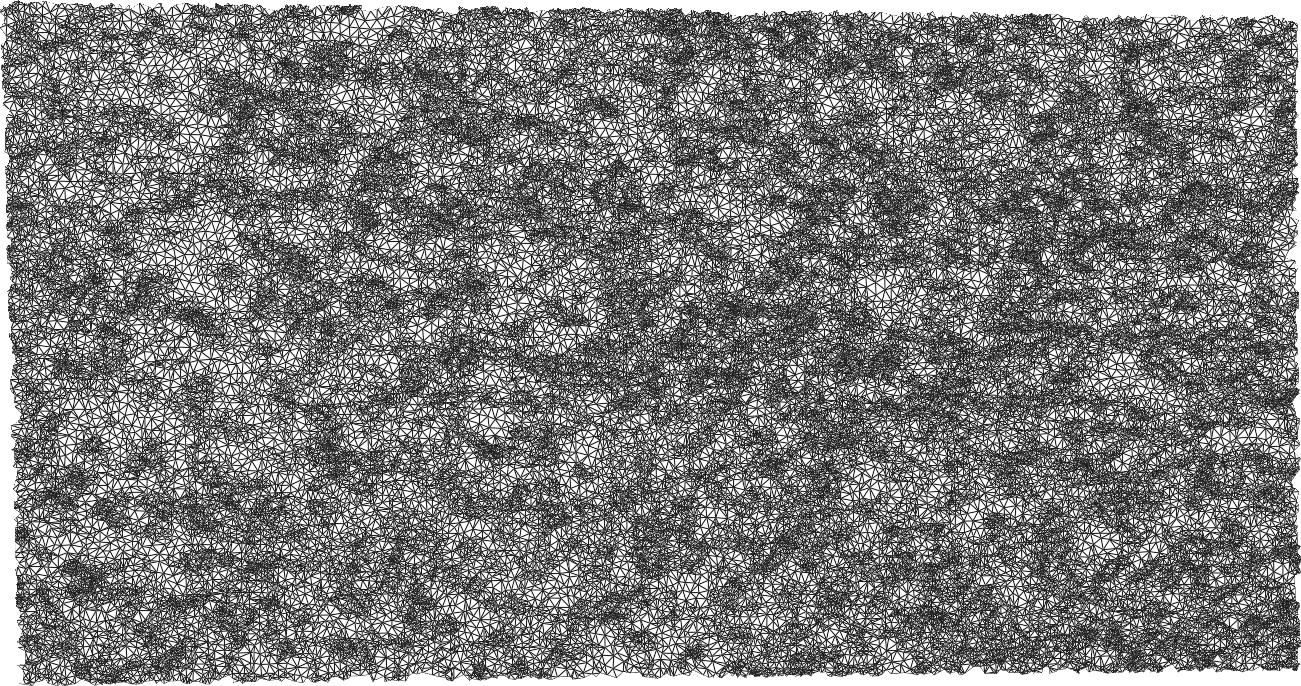
\includegraphics[width=\linewidth]
		{data/acquired_meshes/ILATO_1A_SM2066-HE5-60_070214_merged_GMO_r1_n4_v256_wireframe.png}
		\caption{wireframe}\label{ILATO:bun.a}
	\end{subfigure}
	\begin{subfigure}[b]{0.49\linewidth}
		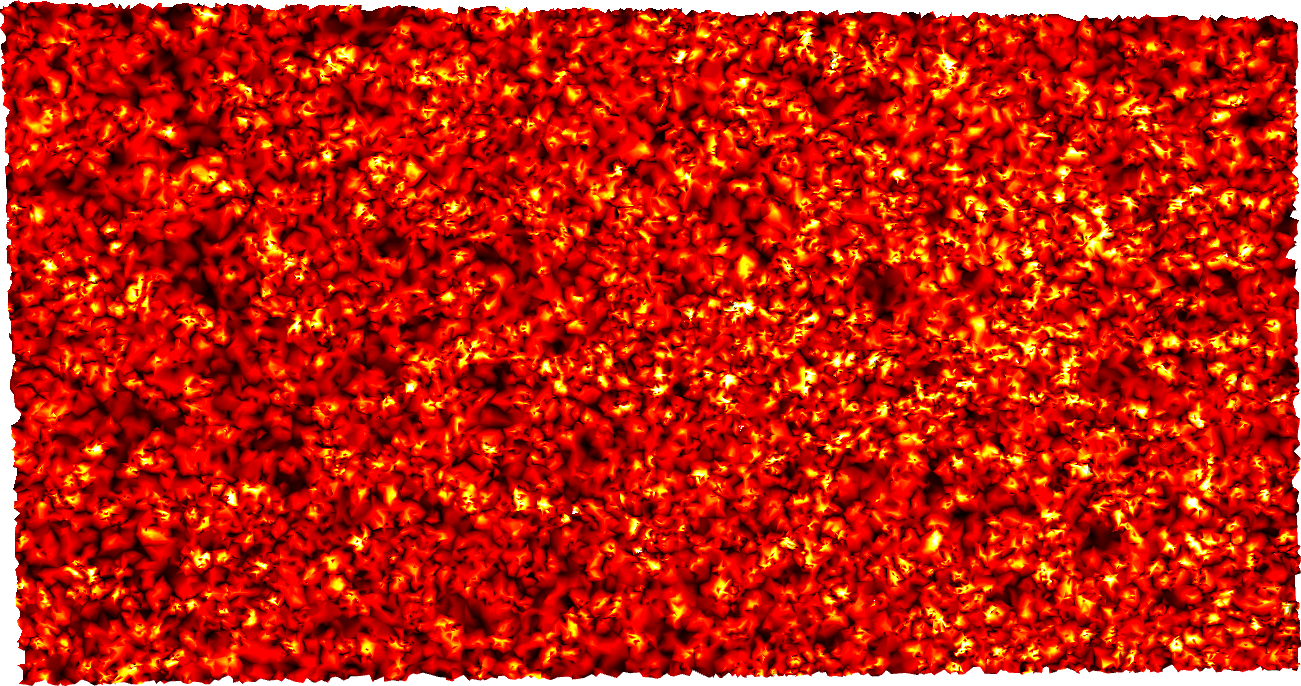
\includegraphics[width=\linewidth]
		{data/acquired_meshes/ILATO_1A_SM2066-HE5-60_070214_merged_GMO_r1_n4_v256_funcvals_0iter.png}
		\caption{$c=0$}\label{fig:buILATOn.b}
	\end{subfigure}

	\bigskip
	\begin{subfigure}[b]{0.49\linewidth}
		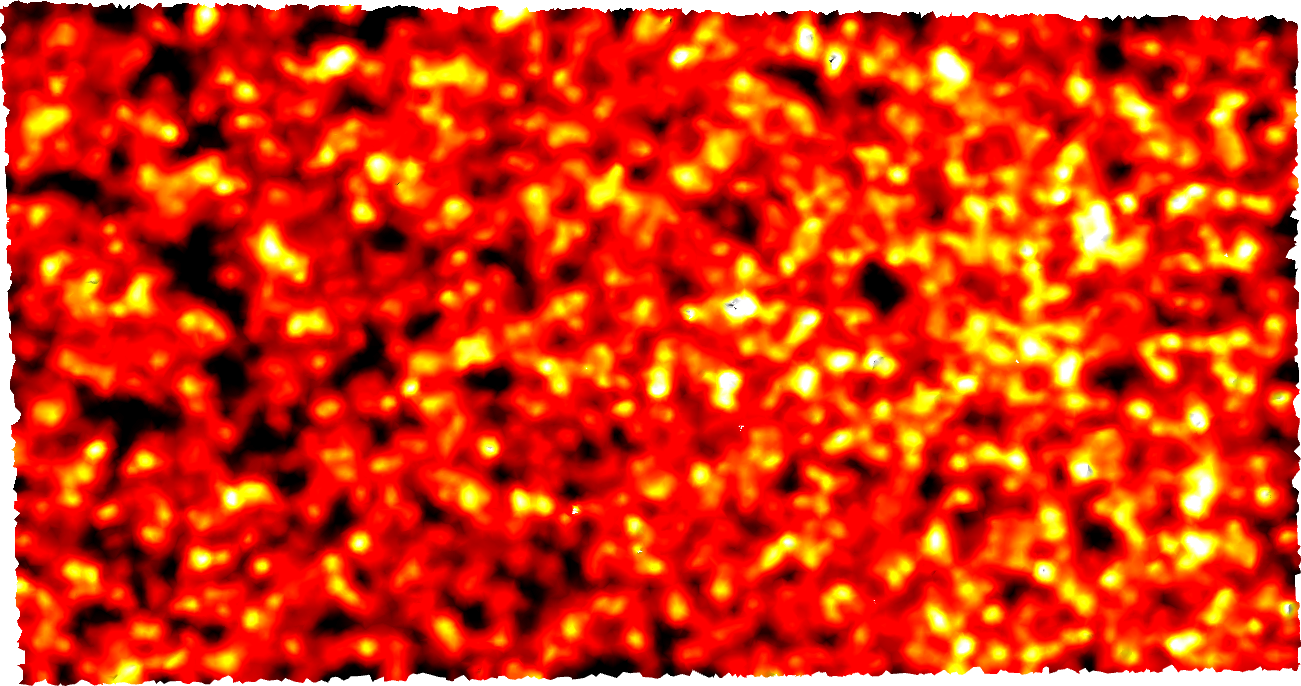
\includegraphics[width=\linewidth]
		{data/acquired_meshes/ILATO_1A_SM2066-HE5-60_070214_merged_GMO_r1_n4_v256_funcvals_1000iter.png}
		\caption{$c=1000$}\label{fig:ILATO.c}
	\end{subfigure}
	\begin{subfigure}[b]{0.49\linewidth}
		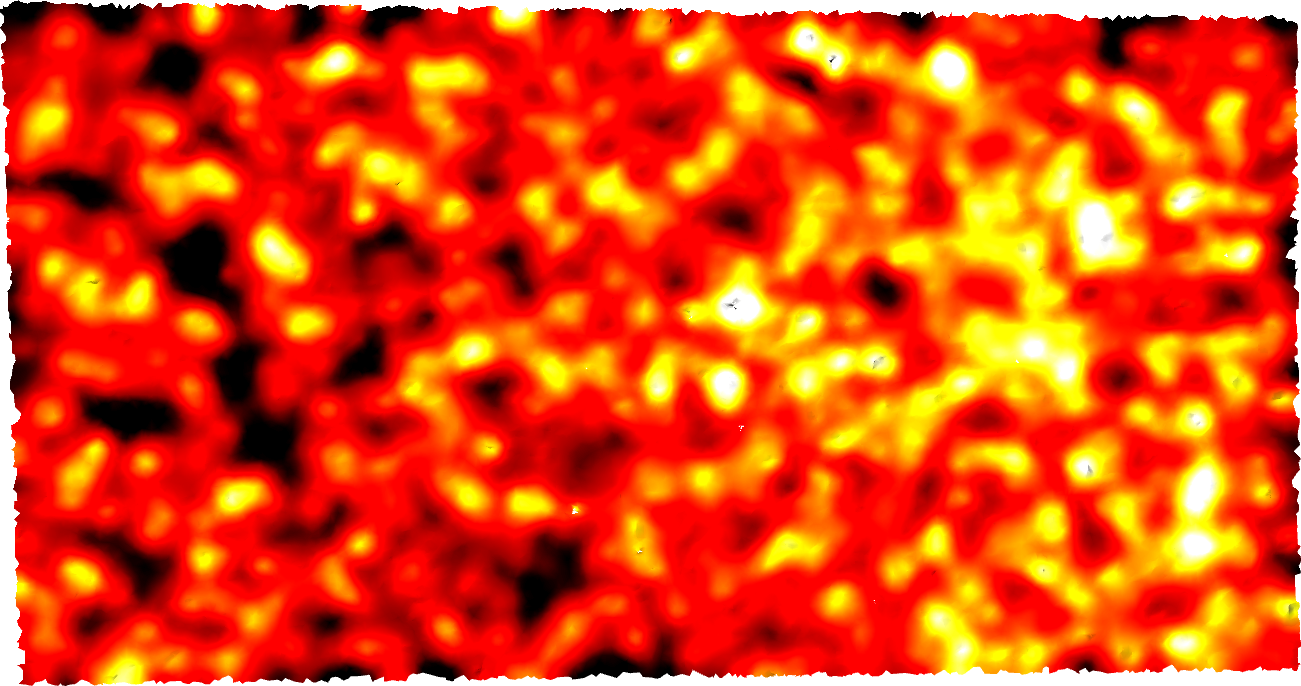
\includegraphics[width=\linewidth]
		{data/acquired_meshes/ILATO_1A_SM2066-HE5-60_070214_merged_GMO_r1_n4_v256_funcvals_3000iter.png}
		\caption{$c=3000$}\label{fig:ILATO.d}
	\end{subfigure}
	\caption[Four Views of the Flat Surface from ILATO]{Four views of a flat surface (a) in wireframe (b) colored by MSII function value before convolving the filter (c) colored by function value after convolving the filter 1,000 times (c) and after 3,000 times.}
	\label{fig:ILATO}
\end{figure}


%
%
%
%
\subsection{Stanford Bunny}
The Stanford Bunny was range scanned in 1994 using a Cyberware 3030MS optical triangulation scanner. The ten separate scans were then zippered together~\cite[Turk94] to produce the \tdd{} which we obtained from The Stanford 3D Scanning Repository~\cite{StanfordBun}. This mesh is comprised of 35,947 points and 69,451 faces.

Figure~\ref{fig:unisiegel} shows\dots
\begin{figure}[ht]
	\begin{subfigure}[b]{0.32\linewidth}
		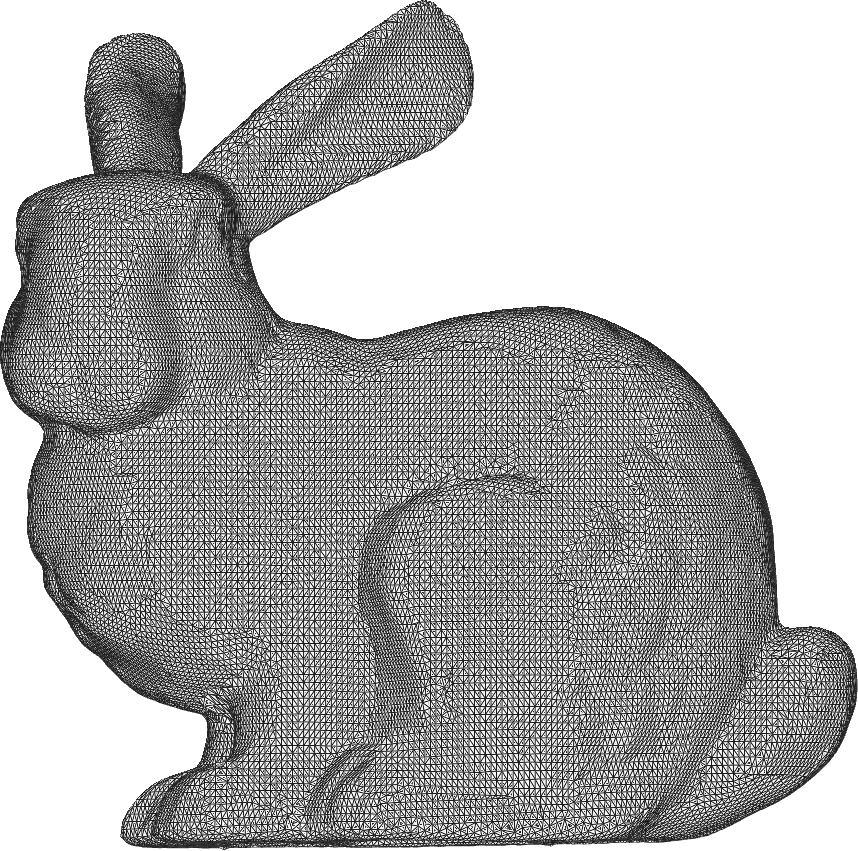
\includegraphics[width=\linewidth]
		{data/acquired_meshes/bun_zipper_edited_r1_n4_v256_wireframe.png}
		\caption{wireframe}\label{fig:bun.a}
	\end{subfigure}
	\begin{subfigure}[b]{0.32\linewidth}
		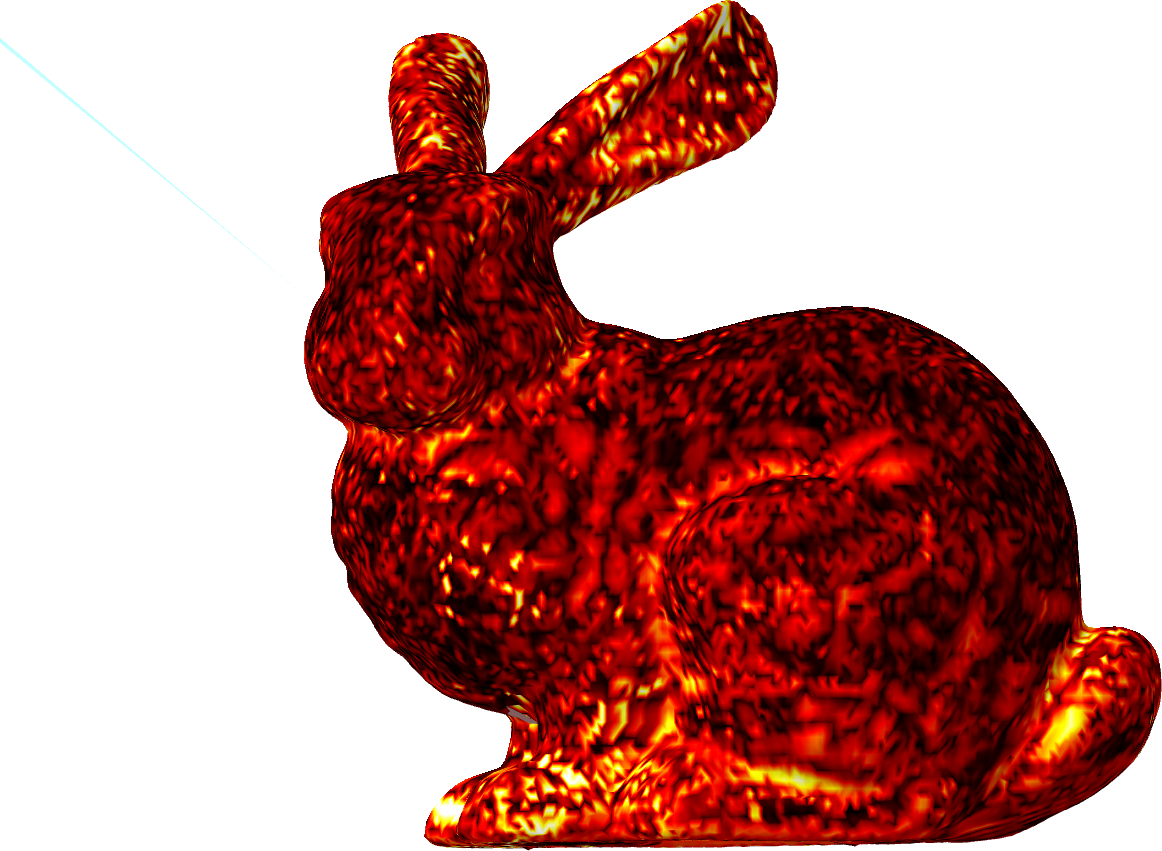
\includegraphics[width=\linewidth]
		{data/acquired_meshes/bun_zipper_edited_r1_n4_v256_funcvals_0iter.png}
		\caption{$c=0$}\label{fig:bun.b}
	\end{subfigure}
	\begin{subfigure}[b]{0.32\linewidth}
		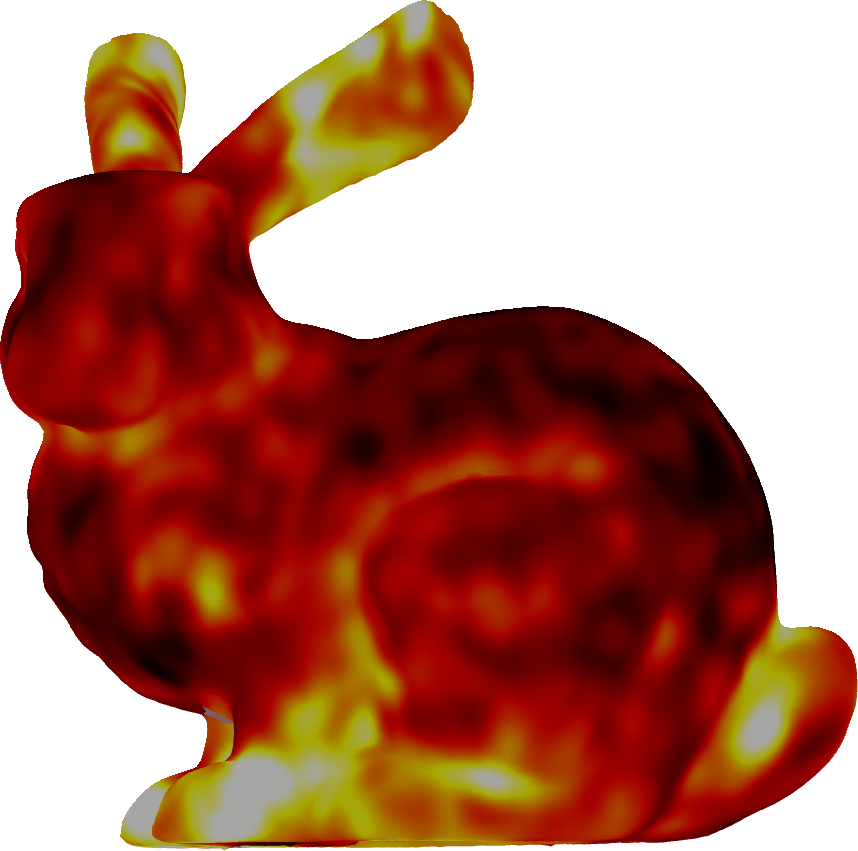
\includegraphics[width=\linewidth]
		{data/acquired_meshes/bun_zipper_edited_r1_n4_v256_funcvals_100iter.png}
		\caption{$c=100$}\label{fig:bun.c}
	\end{subfigure}
	\caption[Three Views of the Stanford Bunny]{Three views of the Stanford Bunny (a) in wireframe, (b) colored by \gls{tMSIIf} value before convolving the filter, and (c) colored by function value after convolving the filter 100 times.}
	\label{fig:bun}
\end{figure}


%
%
%
%
%
%
\section{Evaluation}
\ldots

%
%
%
%
\subsection{Compute Times}

Figure~\ref{fig:computeTimesLP} shows how compute times increase linearly with both mesh size and number of iterations in a very predictable way when total compute time is at least 0.1 seconds, and less predictable for shorter periods do to the nature of thread optimization at the processor level and variable memory read times.\todoResearch{add formula for timing (or at least ref to it) here.}\todoResearch{process time noise at very fast speeds}
\begin{figure}[ht]
	\centering
	\includegraphics[width=1.0\linewidth,height=1.0\textheight,keepaspectratio]
		{figures/computeTimesLinespoints.png}
	\RawCaption{\caption[Compute Times - Linespoints]{Compute Times of Applying
		the	One-Ring Filter for Selected Numbers of Iterations onto Acquired and
		Synthetic 3D Meshes of Varying Sizes}
		\label{fig:computeTimesLP}}
\end{figure}

Figure~\ref{fig:computeTimesS} shows how compute times increase with both meshsize and number of iterations.\todoCitation{wikipedia Euler characteristic Polyhedra}
\begin{figure}[ht]
	\centering
	\includegraphics[width=1.0\linewidth,height=1.0\textheight,keepaspectratio]{figures/computeTimesScatter.png}
	\RawCaption{\caption[Compute Times - Scatter]{Compute Times for Different
		Hardware Configurations by increaseing Mesh Size and Filter Iterations}
		\label{fig:computeTimesS}}
\end{figure}

%
%
%
%
\subsection{Curious Trend, ratio goes to 2}

\begin{figure}[ht]
	\centering
	\includegraphics[width=1.0\linewidth,height=1.0\textheight,keepaspectratio]{figures/numFacesByVerticesGoTo2.png}
	\RawCaption{\caption[Ratio of Faces / Vertices]{Ratio of Faces to Vertices by
		Increasing Vertex Count}
		\label{fig:ratioFacesVertices}}
\end{figure}

%
%
%
%
%
%
\section{Summary}
\dots
